\documentclass{beamer}
\usetheme{Singapore}
%\setbeamercolor{structure}{fg=red}
\usepackage{upgreek}
\usepackage{color}
%\def\magyarOptions{hyphenation=huhyphn}
%\usepackage{ae,aecompl}
%\usepackage[T1]{fontenc}
\usepackage[utf8]{inputenc}
%\usepackage[hungarian]{babel}
\usepackage{gensymb}
\usepackage{pgfplots}
\usepackage{pst-plot}
\usepackage{tikz}
\usepgfplotslibrary{external}
\tikzexternalize
\usepackage[version=3]{mhchem}
\usepackage{listings}

\normalfont
\title{Deconvolution in Scanning Electrochemical Microscopy}
\author
{
Dr. András Kiss\\
}

\institute
{
  %\inst{1}%
  Department of General and Physical Chemistry\\
  University of Pécs, Hungary\\
    \hfill \\

  
\includegraphics[width=0.14\textwidth]{pte_logo.eps}\\
  \vspace{0.1cm}
  Center for Integrative Physiology\\
  and Molecular Medicine\\
  Universität des Saarlandes, Homburg, Germany
  
  
\includegraphics[width=0.2\textwidth]{cipmm.png}\\

  %June 16, 2017
}

\date[]

\begin{document}
\frame{\titlepage}  

\begin{frame}[plain]
	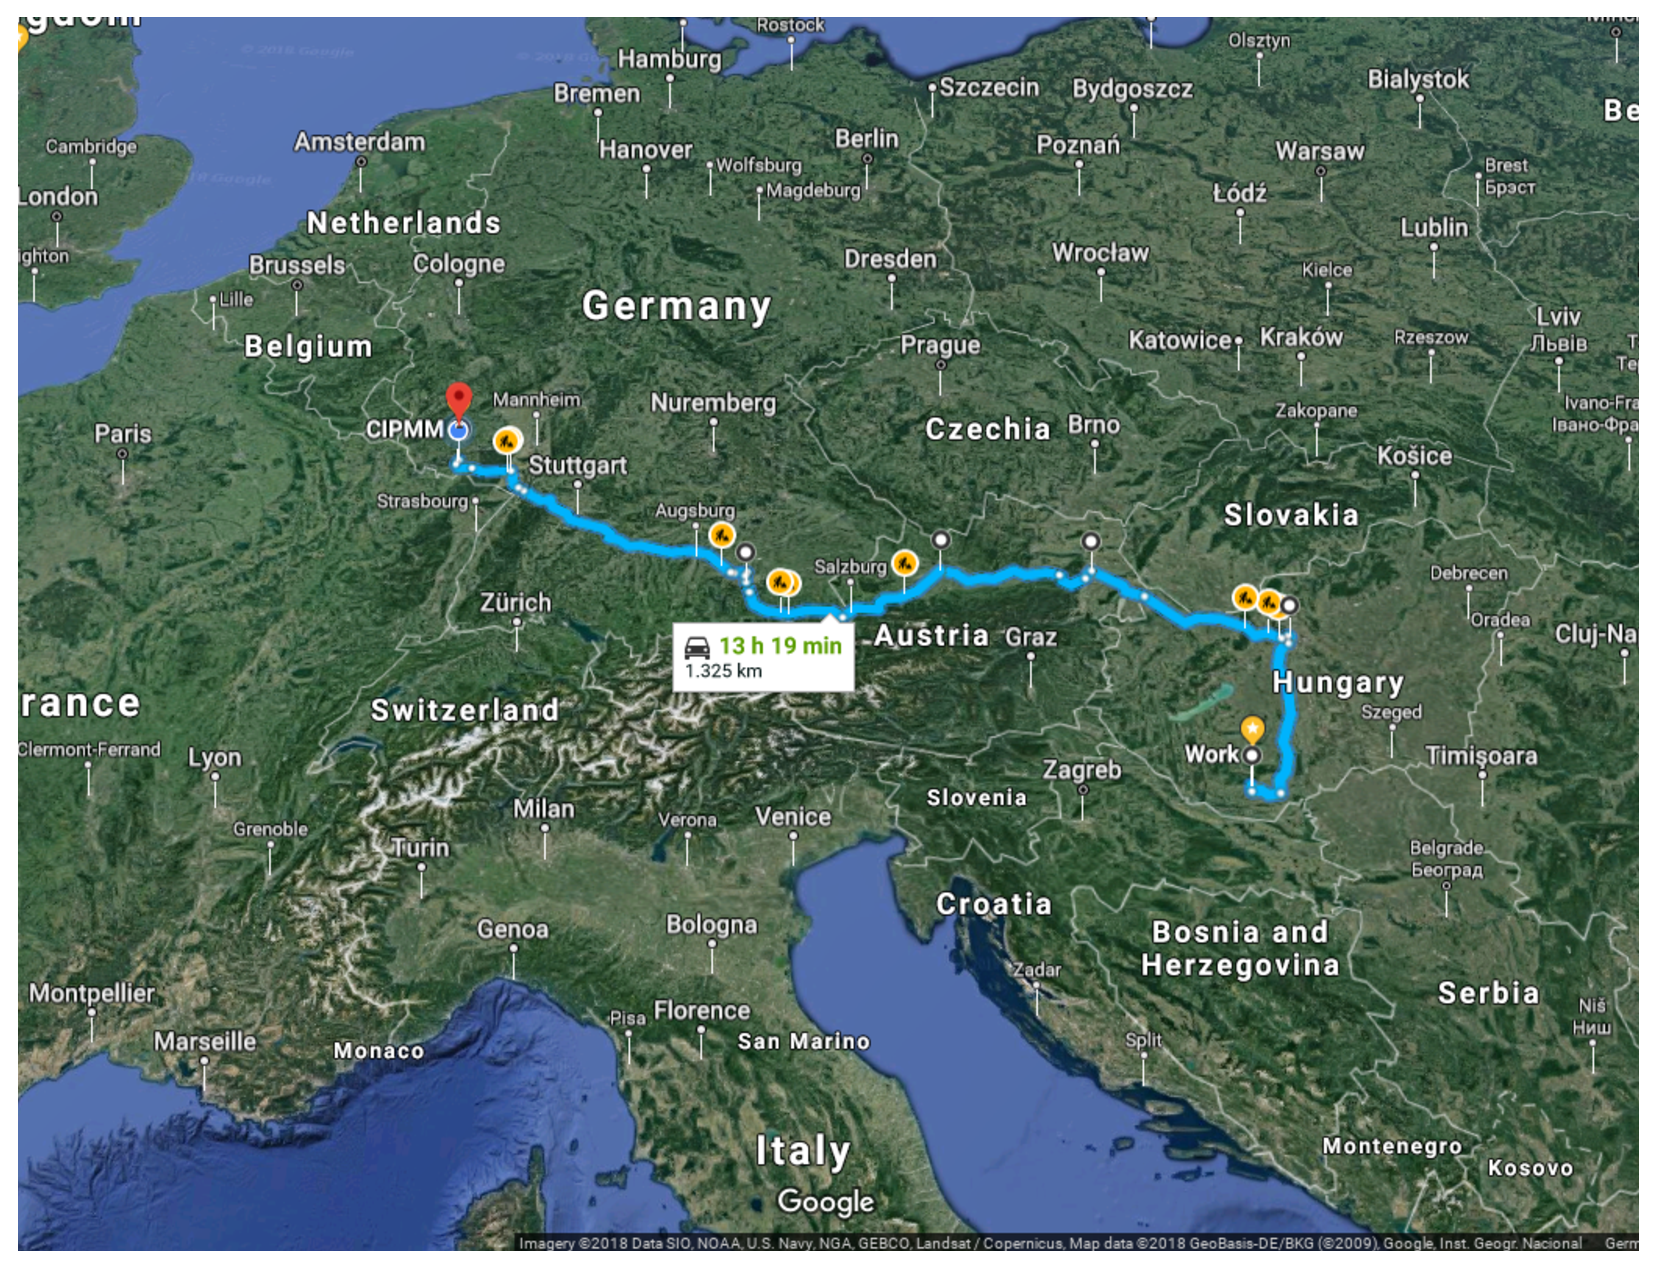
\includegraphics[width=1\textwidth]{journey.eps}
\end{frame}

\begin{frame}[plain]
	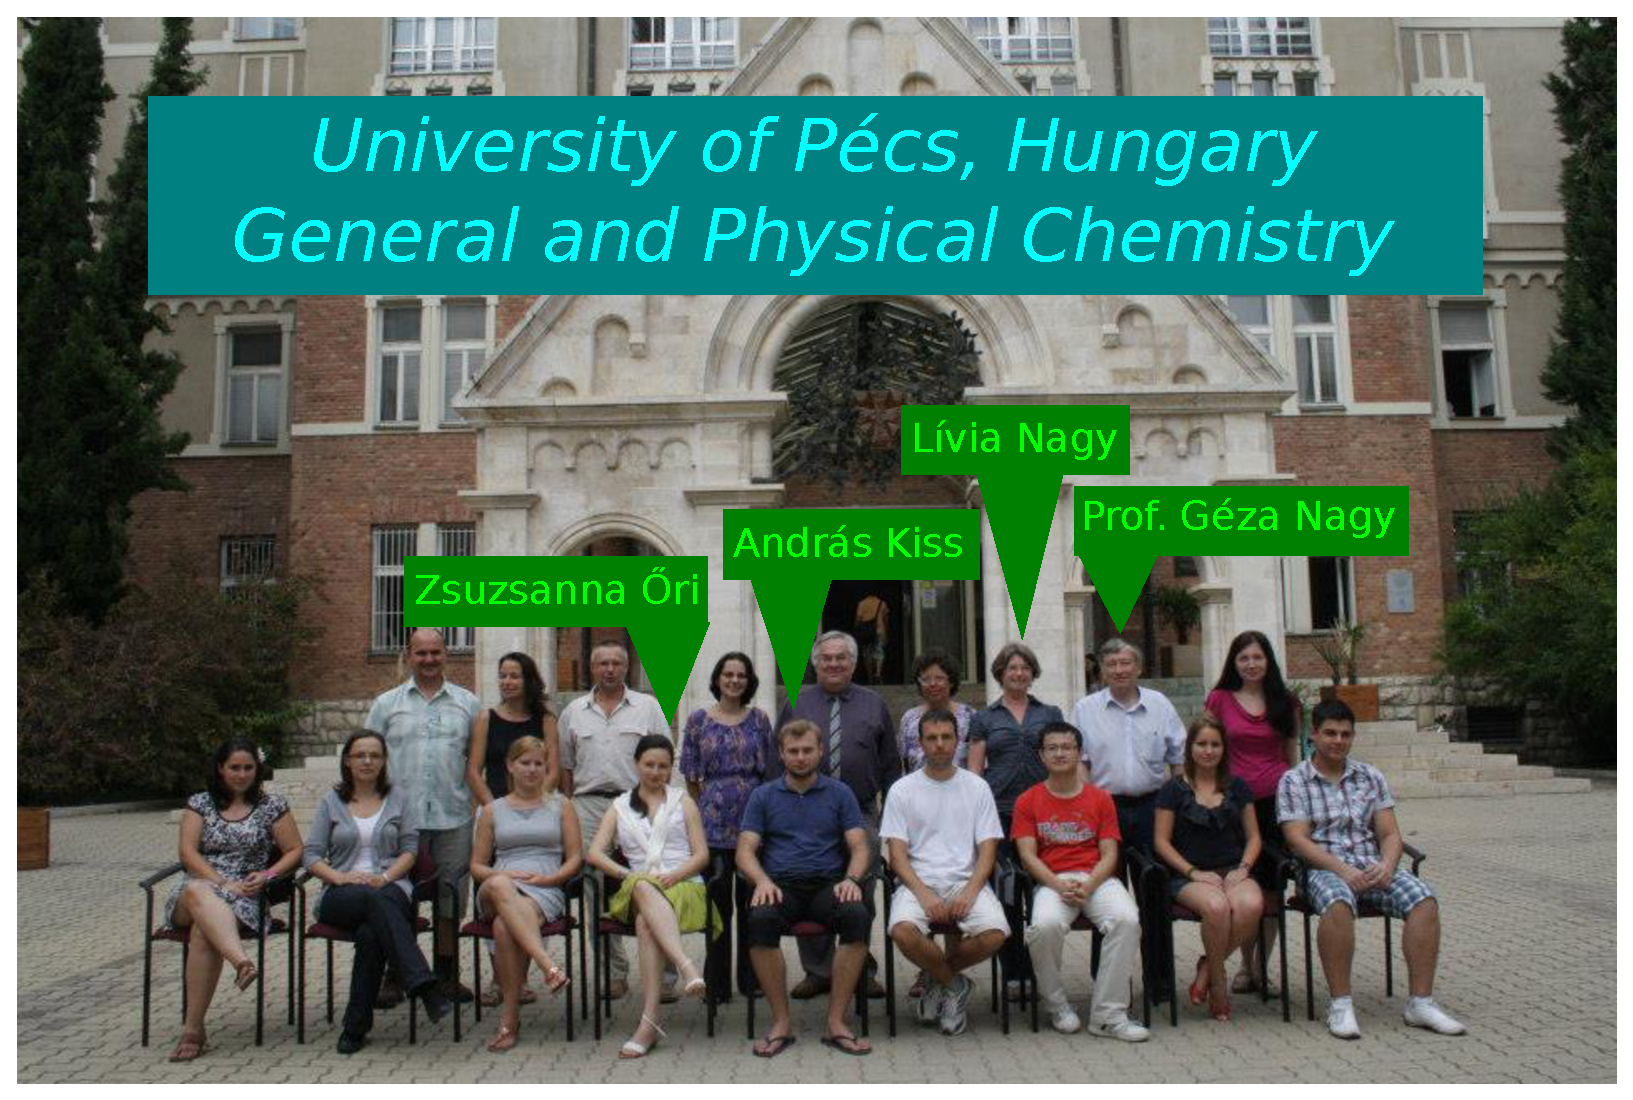
\includegraphics[width=1\textwidth]{fizkem.eps}
\end{frame}


\begin{frame}
	\centering
	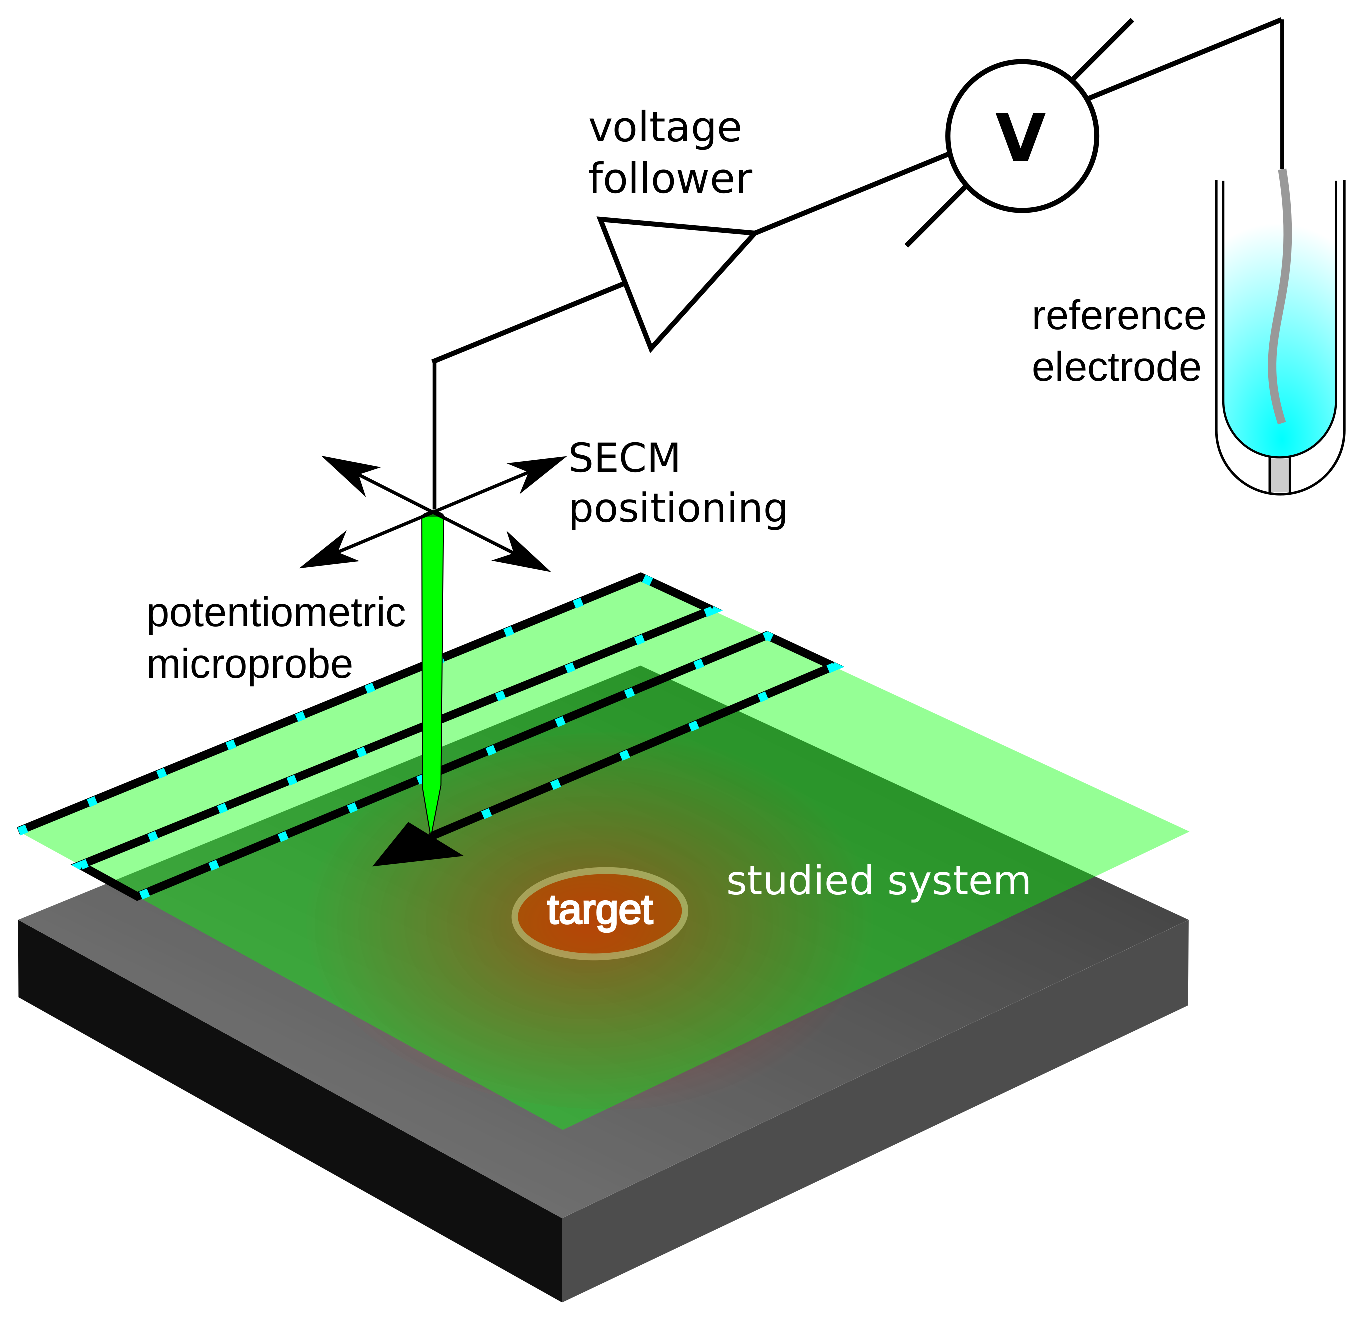
\includegraphics[width=0.6\textwidth]{secm.eps}
	\frametitle{Potentiometric \underline{S}canning \underline{E}lectro\underline{c}hemical \underline{M}icroscopy}
	\framesubtitle{A Scanning Probe Microscopic technique}
\end{frame}

\begin{frame}
	\centering
	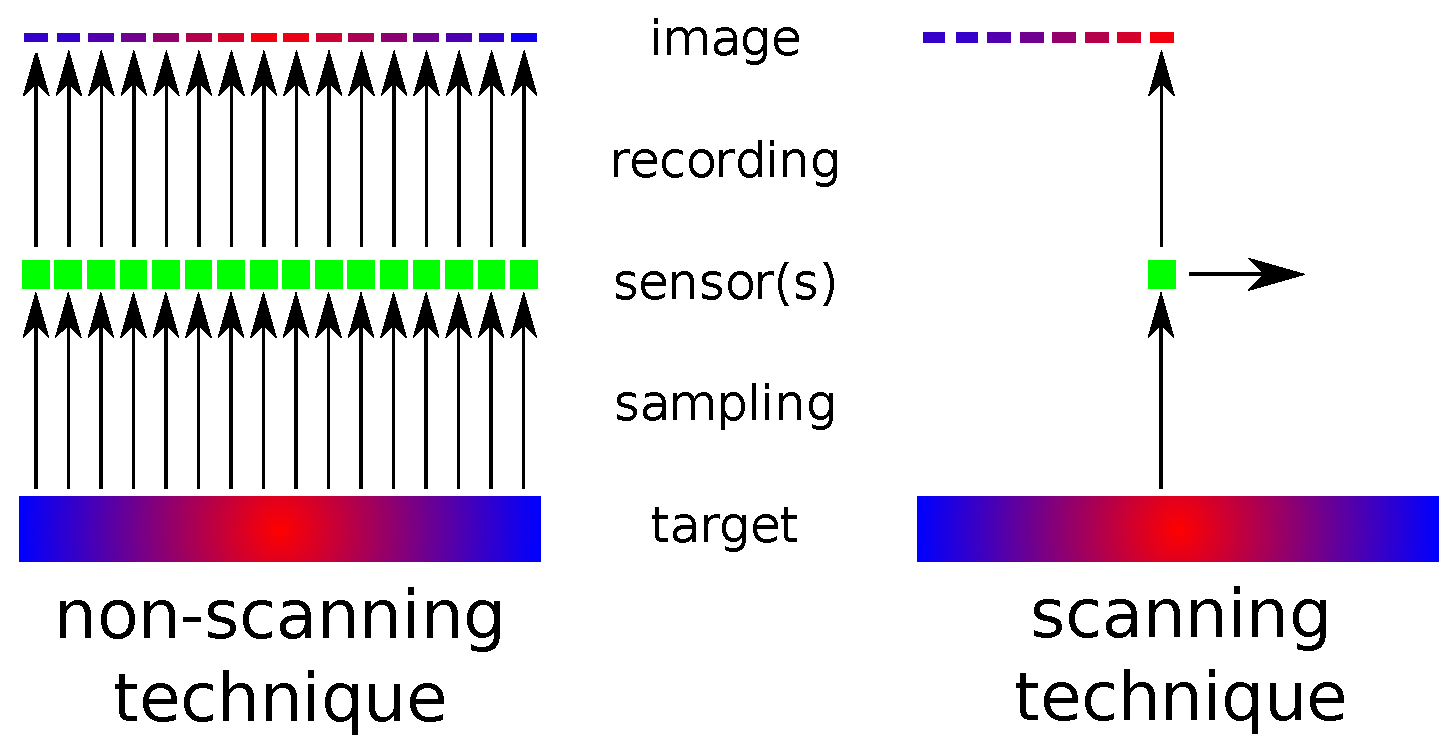
\includegraphics[width=0.9\textwidth]{microscopy.eps}
	\frametitle{Difference between conventional and scanning microscopic techniques}
\end{frame}



\begin{frame}
\frametitle{Ion-selective micropipettes}
\framesubtitle{As SECM probes}
\begin{columns}[T] % align columns
\begin{column}{.48\textwidth}

\centering
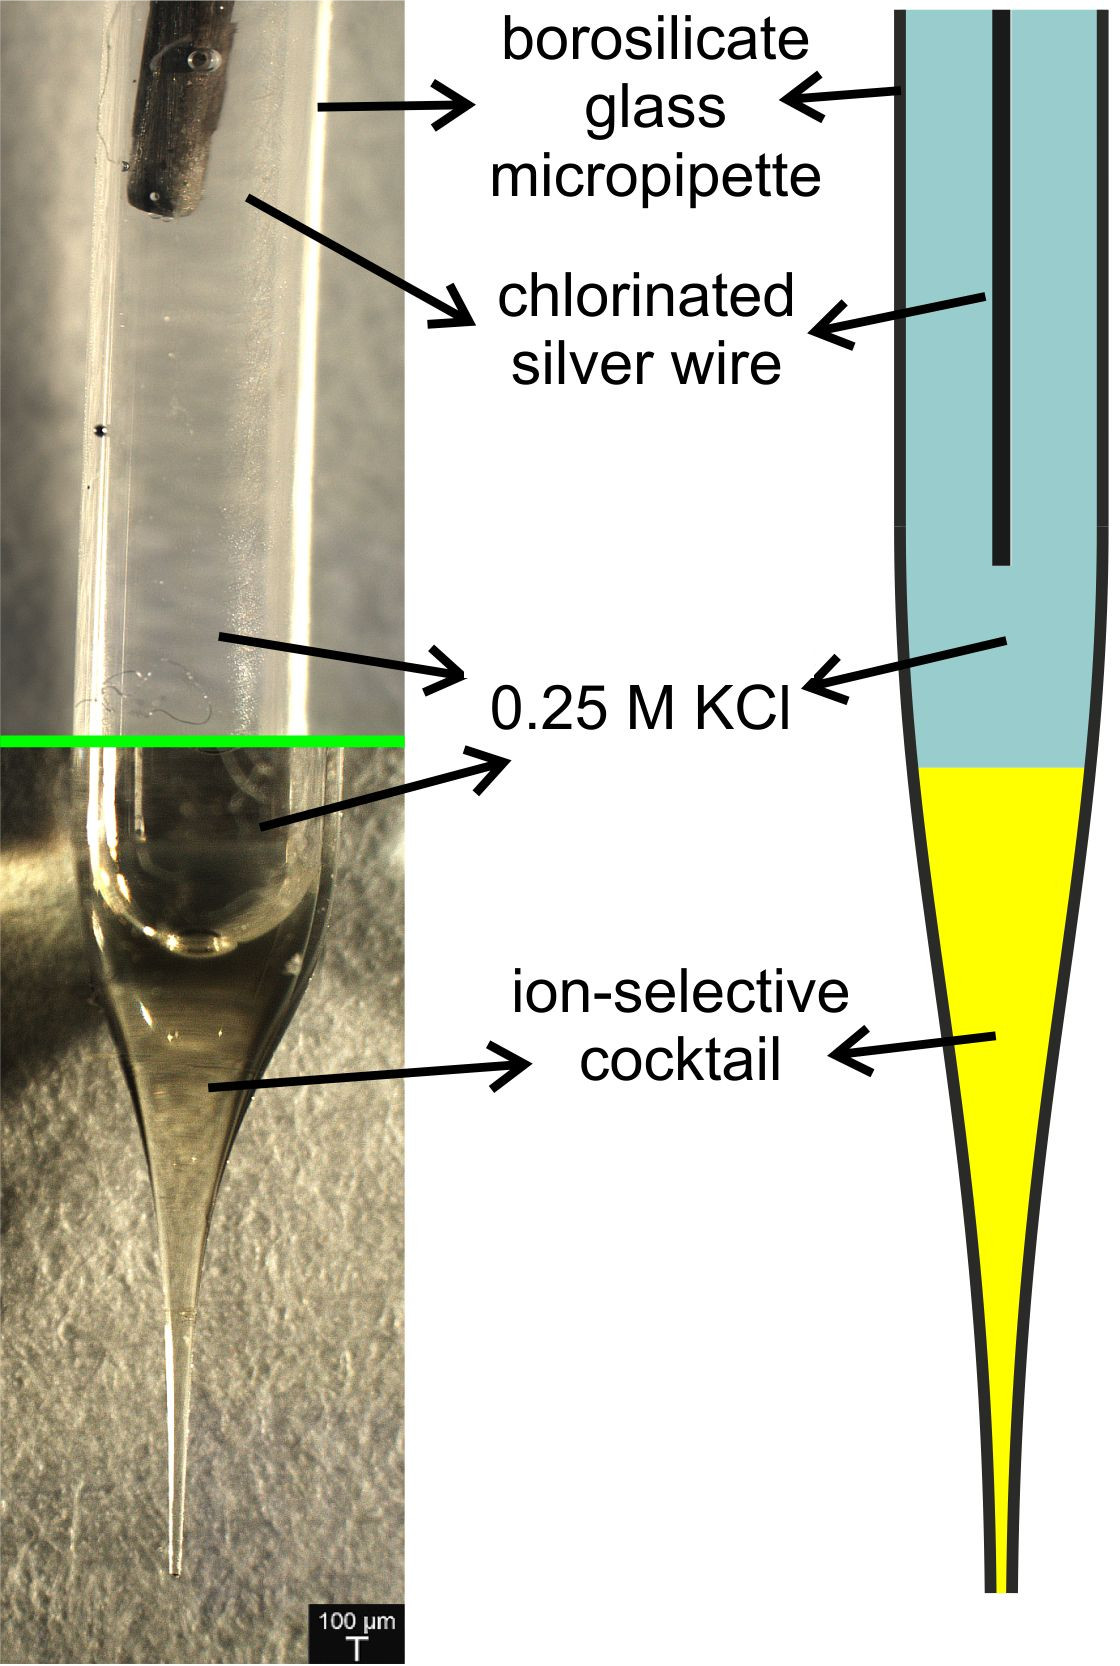
\includegraphics[width=0.9\textwidth]{liquid.jpg}
\end{column}%
\hfill%
\begin{column}{.48\textwidth}
%\color{blue}\rule{\linewidth}{4pt}
\centering

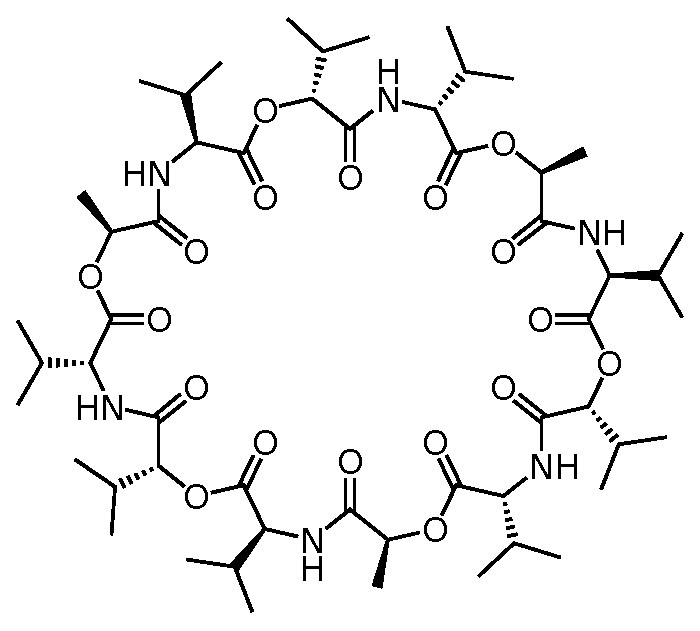
\includegraphics[width=0.8\textwidth]{Valinomycin.eps}

Valinomycin
\vfill

\footnotesize
\begin{equation*}
        E=E^\theta + \frac{RT}{z_iF} \ln \left [ a_i + \sum_{j} \left ( k_{ij}a_j^{z_i/z_j} \right ) \right ]
        \end{equation*}
\normalsize
Nikolsky--equation
\end{column}%
\end{columns}
\end{frame}

\begin{frame}
	\frametitle{The problem with potentiometric SECM} 
	\framesubtitle{Distortion at high scan rate}
	\centering
\quad\quad\quad\quad\quad\quad Slow \hfill Fast \quad\quad\quad\quad\quad\quad\quad

	\includegraphics[trim = 10mm 30mm 0mm 20mm, clip, width=0.4\textwidth, angle=-90]{real.eps}\hfill\includegraphics[trim = 10mm 30mm 0mm 20mm, clip, width=0.4\textwidth, angle=-90]{fastcomb_sim.eps}
\end{frame}

\begin{frame}
\frametitle{Why is the image distorted?}
\framesubtitle{Possible contributors to the lag}
\centering
\includegraphics[width=0.8\textwidth]{npp.eps}
\end{frame}

\begin{frame}
	\frametitle{Why is the image distorted?}
	\framesubtitle{The RC time constant} 
	\centering
	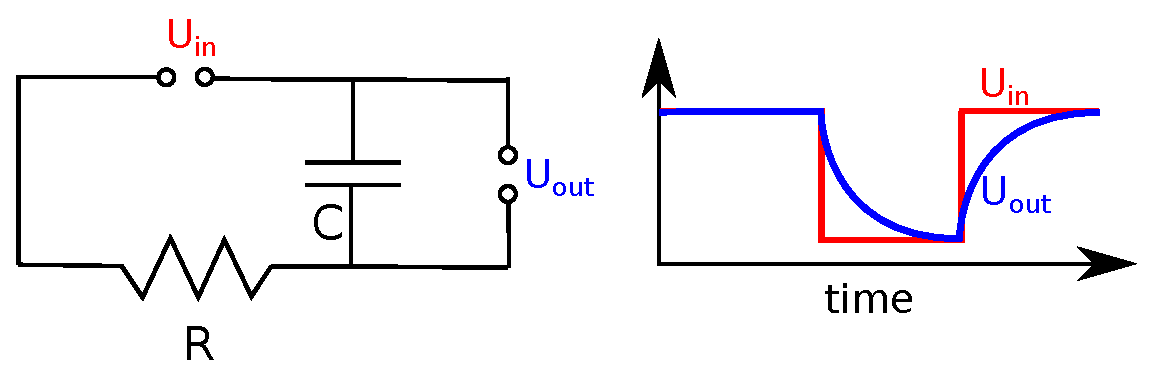
\includegraphics[width=1\textwidth]{RC.eps}
	\vfill
	$\tau$ is the time that is required to charge \\ the capacitor by $\approx 37\%$ $(1/e)$.	
%	\vfill
%	$\tau = R \cdot C$
%	
%	$R = 5 $ G$\ohm$
%	
%	$C = 500 $ pF
%	
%	\textbf{\textcolor{white!100}{\colorbox{red!100}{$\tau = 2.5 $ s}}}

	%\includegraphics[width=0.6\textwidth, angle=-90]{meander_sim.eps}
\end{frame}

\begin{frame}
	\frametitle{Distortion of potentiometric imaging} 
	\framesubtitle{In the case of a linescan} 
	\centering
	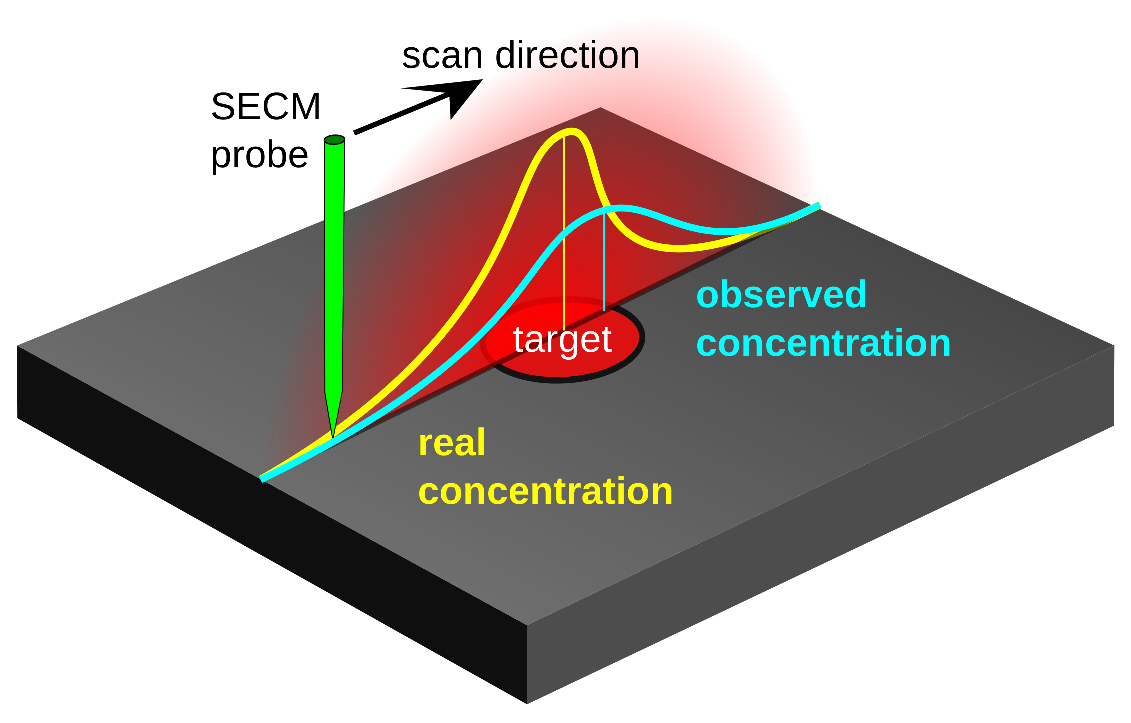
\includegraphics[width=0.8\textwidth]{distortion2.eps}
\end{frame}

%\begin{frame}
%	\frametitle{Why is it so important to complete the scan quickly?}
%	\framesubtitle{Example: corrosion of a magnesium alloy}
%	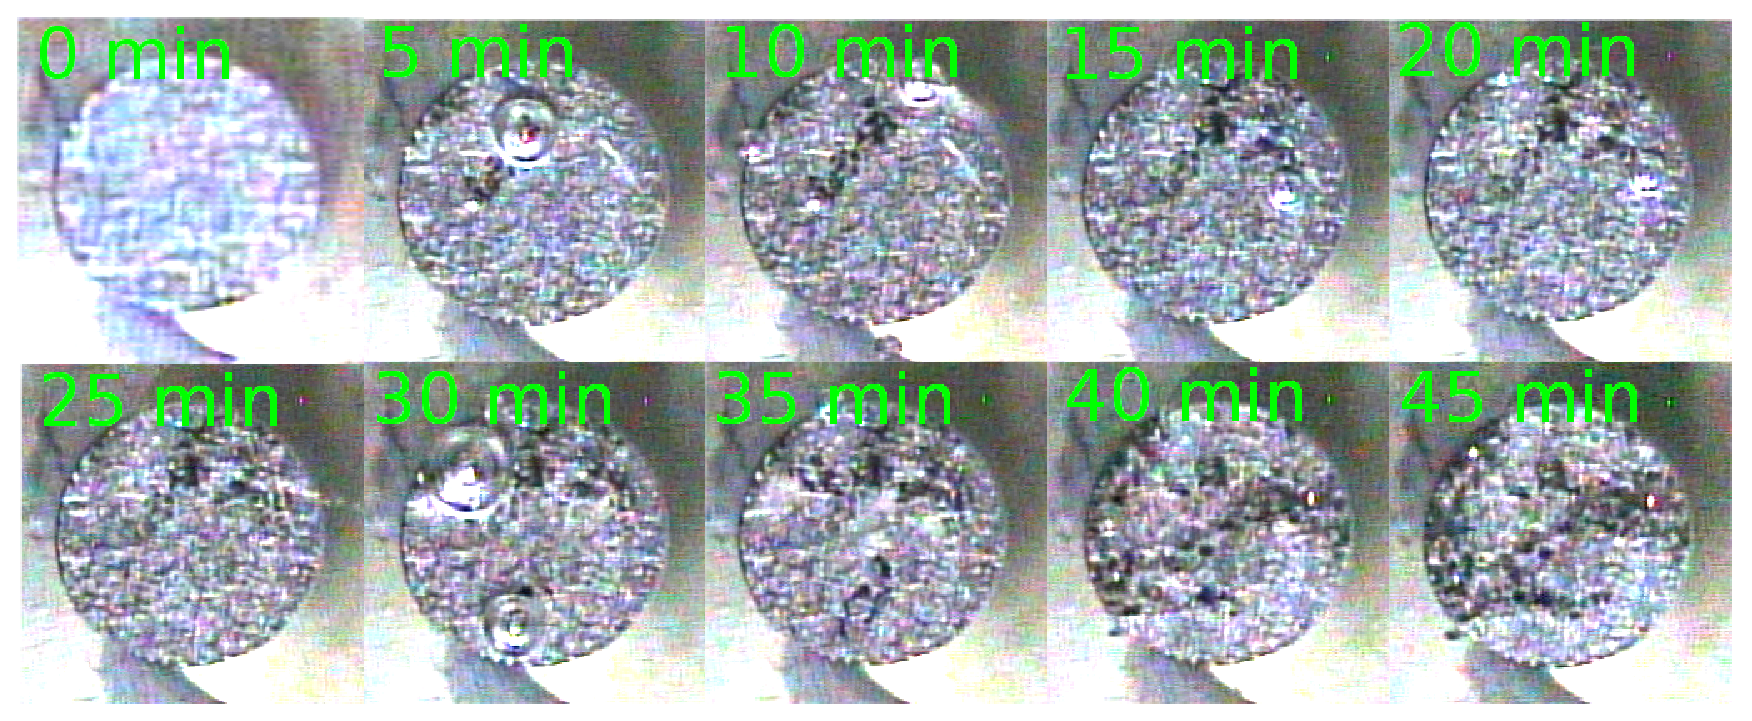
\includegraphics[width=1\textwidth]{timelapse.eps}\\
%\centering
%Corrosion of the AZ63 magnesium-aluminium-zinc alloy.
%%Location of the anodic and cathodic spots change quickly. High-speed scanning is required to complete the scan before the studied system changes.
%\end{frame} 

\begin{frame}
\frametitle{Trade-off triangle of potentiometric SECM}
\framesubtitle{Compromise between the three desired competing properties}
\begin{center}
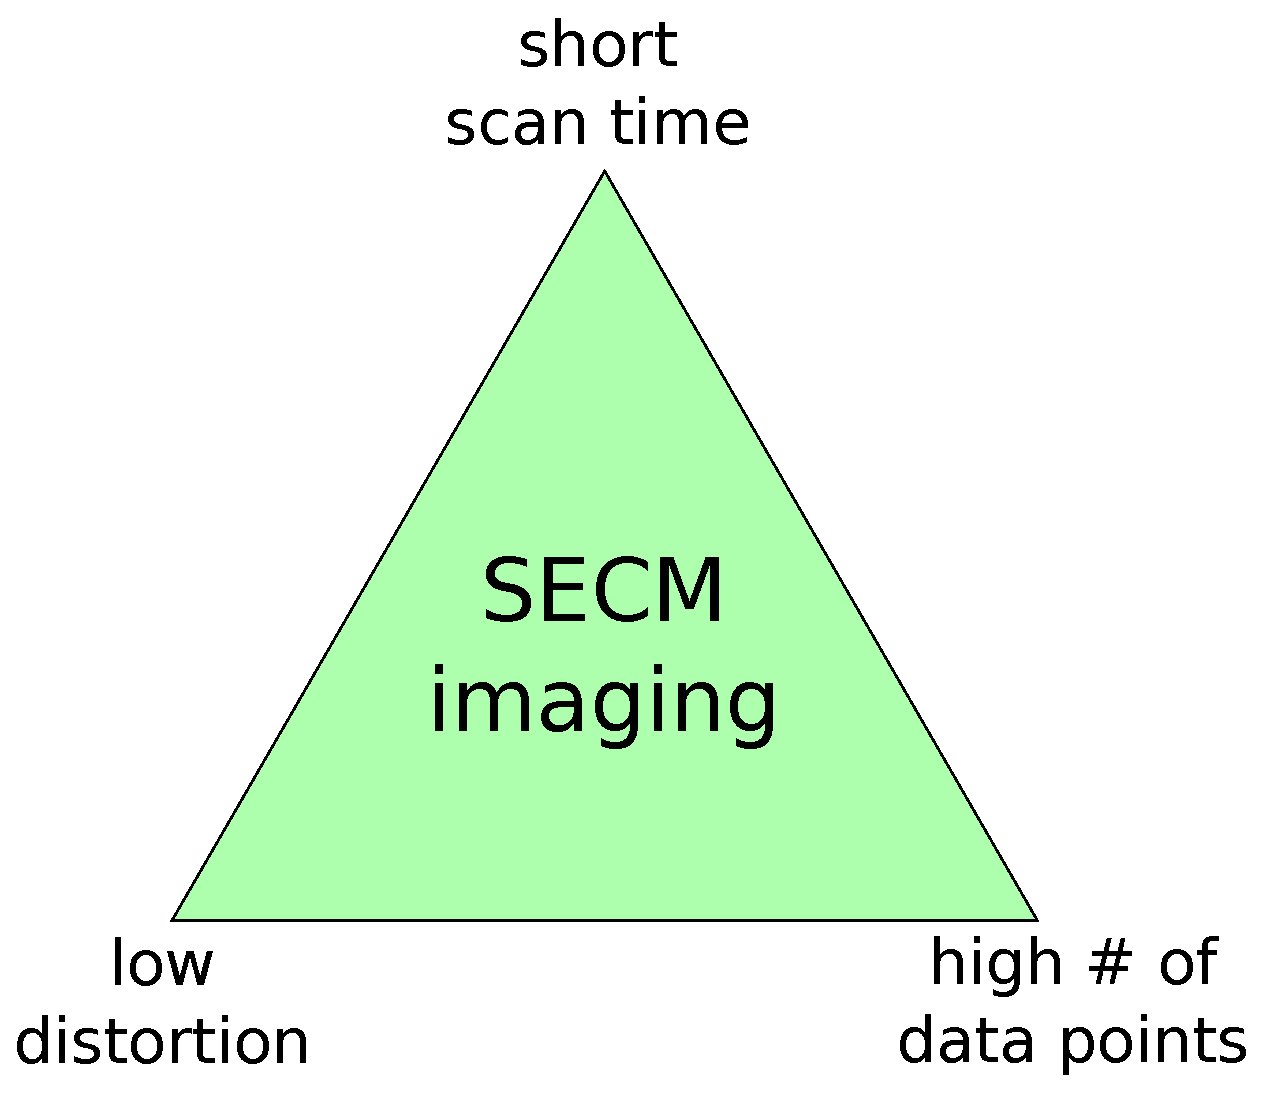
\includegraphics[width=0.5\textwidth]{trade-off.eps}
\end{center}
\end{frame}

\begin{frame}
\frametitle{The convolution function of the distortion}
\centering	
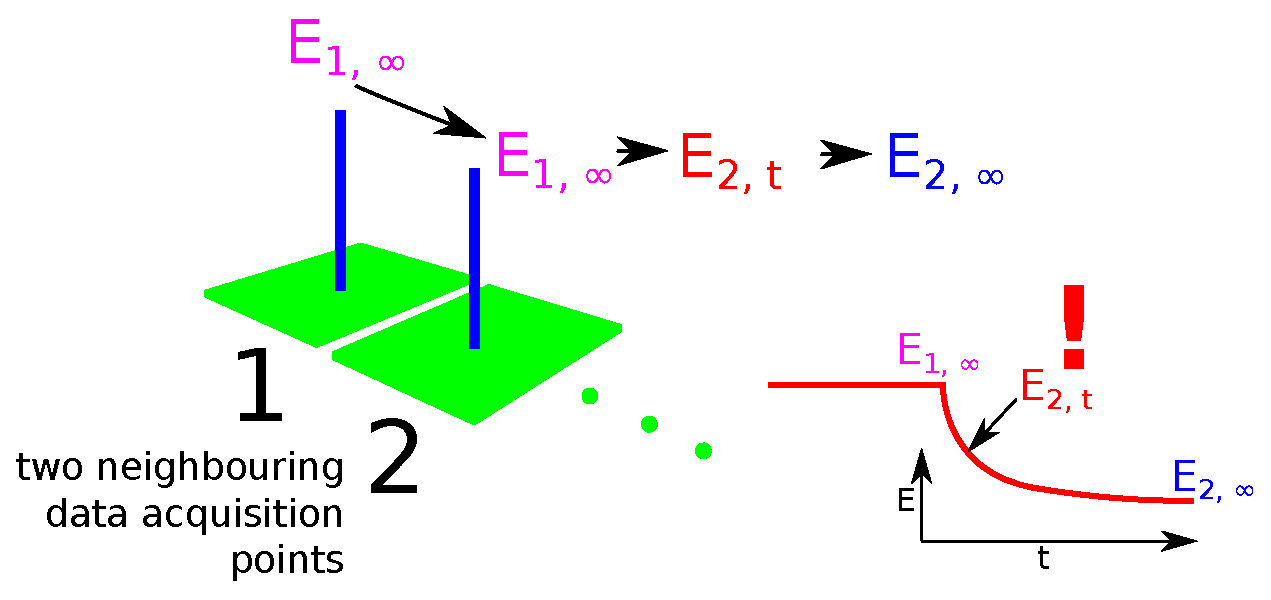
\includegraphics[width=1\textwidth]{t.eps}\\
\vfill
$E_{cell}(t) = E_{cell}(\infty) + [E_{cell}(0) - E_{cell}(\infty)]e^{-t/\tau}$\\
\vfill
%$E_{cell}(\infty)	= \frac {\displaystyle [E_{cell}(t) - E_{cell}(0)]e^{-t/RC}}	{\displaystyle 1 - e^{-t/RC}}$
\end{frame}

\begin{frame}
\frametitle{Convolution and deconvolution}
\centering
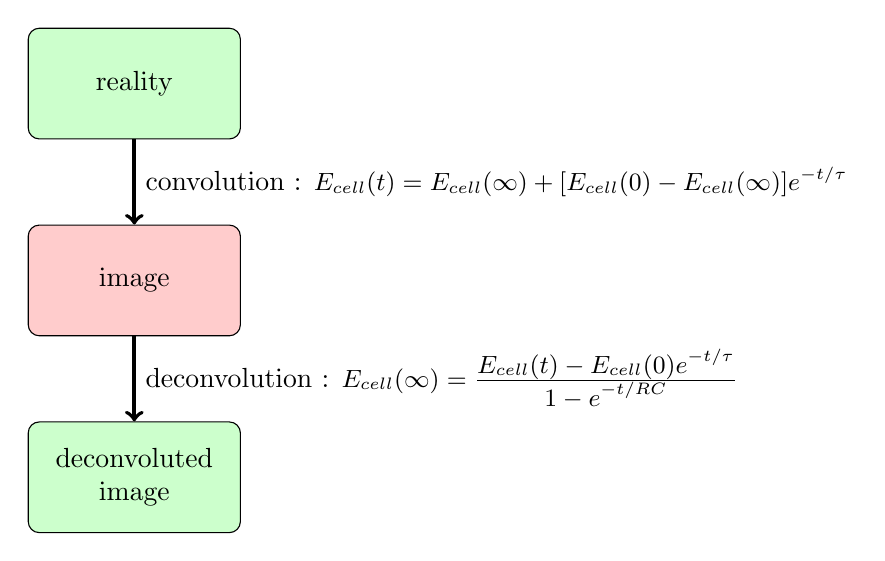
\begin{tikzpicture}[node distance = 2.5cm, auto]
\node [rectangle, draw, fill=green!20,text width=7em, text centered, rounded corners, minimum height=4em] (reality) {reality};
\node [rectangle, below of=reality, draw, fill=red!20,text width=7em, text centered, rounded corners, minimum height=4em] (measurement) {image};
\node [rectangle, below of=measurement, draw, fill=green!20,text width=7em, text centered, rounded corners, minimum height=4em] (image) {deconvoluted\\ image};

\draw [line width=0.5mm, ->] (reality) -- (measurement) node [pos=.5, right] (TextNode) {convolution : \small $E_{cell}(t) = E_{cell}(\infty) + [E_{cell}(0) - E_{cell}(\infty)]e^{-t/\tau}$};
\draw [line width=0.5mm, ->] (measurement) -- (image) node [pos=.5, right] (TextNode) {deconvolution : \small $E_{cell}(\infty)      = \frac {\displaystyle E_{cell}(t) - E_{cell}(0)e^{-t/\tau}}    {\displaystyle 1 - e^{-t/RC}}$};
\end{tikzpicture}
\end{frame}

\begin{frame}
	\frametitle{Deconvolution of potentiometric SECM images}
	\framesubtitle{Recorded using the antimony microelectrode following the meander algorithm}
\centering

\def\s{0.15}

\begin{columns}[T] % align columns

\begin{column}{.2\textwidth}
\begin{minipage}[c][0.75\textheight][c]{\linewidth}
\centering
%raw\\
%images
\end{minipage}
\end{column}%
\hfill%
\begin{column}{.2\textwidth}
\centering
\includegraphics[trim = 10mm 30mm 0mm 10mm, clip, width=0.8\textwidth, angle=-90]{13121313.eps}\\
\includegraphics[trim = 10mm 30mm 0mm 10mm, clip, width=0.8\textwidth, angle=-90]{13121314.eps}\\
\includegraphics[trim = 10mm 30mm 0mm 10mm, clip, width=0.8\textwidth, angle=-90]{13121315.eps}\\
\includegraphics[trim = 10mm 30mm 0mm 10mm, clip, width=0.8\textwidth, angle=-90]{13121316.eps}\\
\end{column}%
\begin{column}{.2\textwidth}
\begin{minipage}[c][0.7\textheight][c]{\linewidth}
\centering
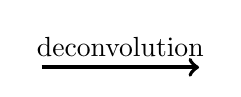
\begin{tikzpicture}
\draw [line width=0.5mm,->] (0,0) -- (2,0) node [pos=.5, above] (TextNode) {deconvolution};
\end{tikzpicture}
\end{minipage}
\end{column}%
\begin{column}{.2\textwidth}
\centering
\includegraphics[trim = 10mm 30mm 0mm 10mm, clip, width=0.8\textwidth, angle=-90]{13121313_deconvoluted.eps}\\
\includegraphics[trim = 10mm 30mm 0mm 10mm, clip, width=0.8\textwidth, angle=-90]{13121314_deconvoluted.eps}\\
\includegraphics[trim = 10mm 30mm 0mm 10mm, clip, width=0.8\textwidth, angle=-90]{13121315_deconvoluted.eps}\\
\includegraphics[trim = 10mm 30mm 0mm 10mm, clip, width=0.8\textwidth, angle=-90]{13121316_deconvoluted.eps}\\
\end{column}%
\begin{column}{.2\textwidth}
\begin{minipage}[c][0.75\textheight][c]{\linewidth}
\centering
%deconvoluted\\
%images
\end{minipage}
\end{column}%
\end{columns}
\end{frame}

\begin{frame}
\frametitle{Practical example: corroding carbon steel sample}
\framesubtitle{Scanned with an antimony microelectrode}
\begin{figure}
\centering
%top left bottom right
\includegraphics[trim = 10mm 30mm 0mm 10mm, clip, width=0.3\textwidth, angle=-90]{16012906.eps}\includegraphics[trim = 10mm 30mm 0mm 10mm, clip, width=0.3\textwidth, angle=-90]{16012906_deconvoluted.eps}

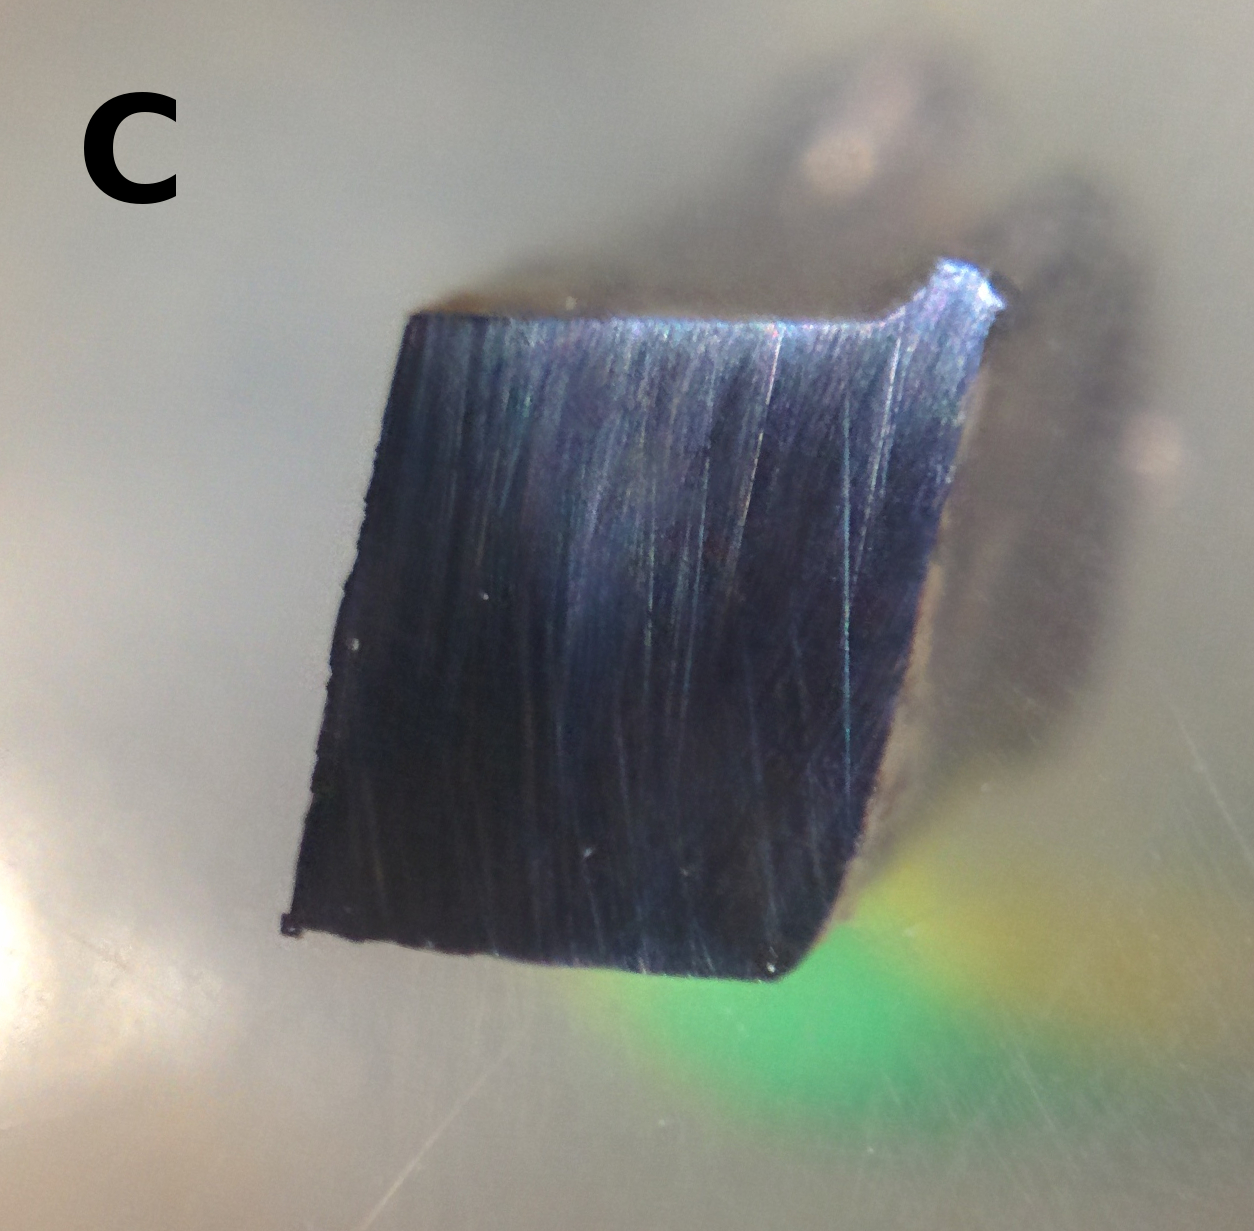
\includegraphics[width=0.24\textwidth]{cs_cut.jpg}

%\caption[Raw, and deconvoluted SECM image and microphoto of a corroding carbon-steel sample polarized anodically.]{Raw (A), and deconvoluted (B) SECM image and microphoto (C) of a corroding carbon-steel sample polarized anodically with a current density of 10 $mA/cm^2$. Measuring electrode was an antimony pH microelectrode. Potential was measured against an Ag/AgCl/3M KCl. Recorded $h$ = 100 $\upmu$m above the surface with probe movement speed of 1000 $\upmu$m/s, equilibration interval 0.4 s.}
\end{figure}
\end{frame}

\begin{frame}
	\centering
	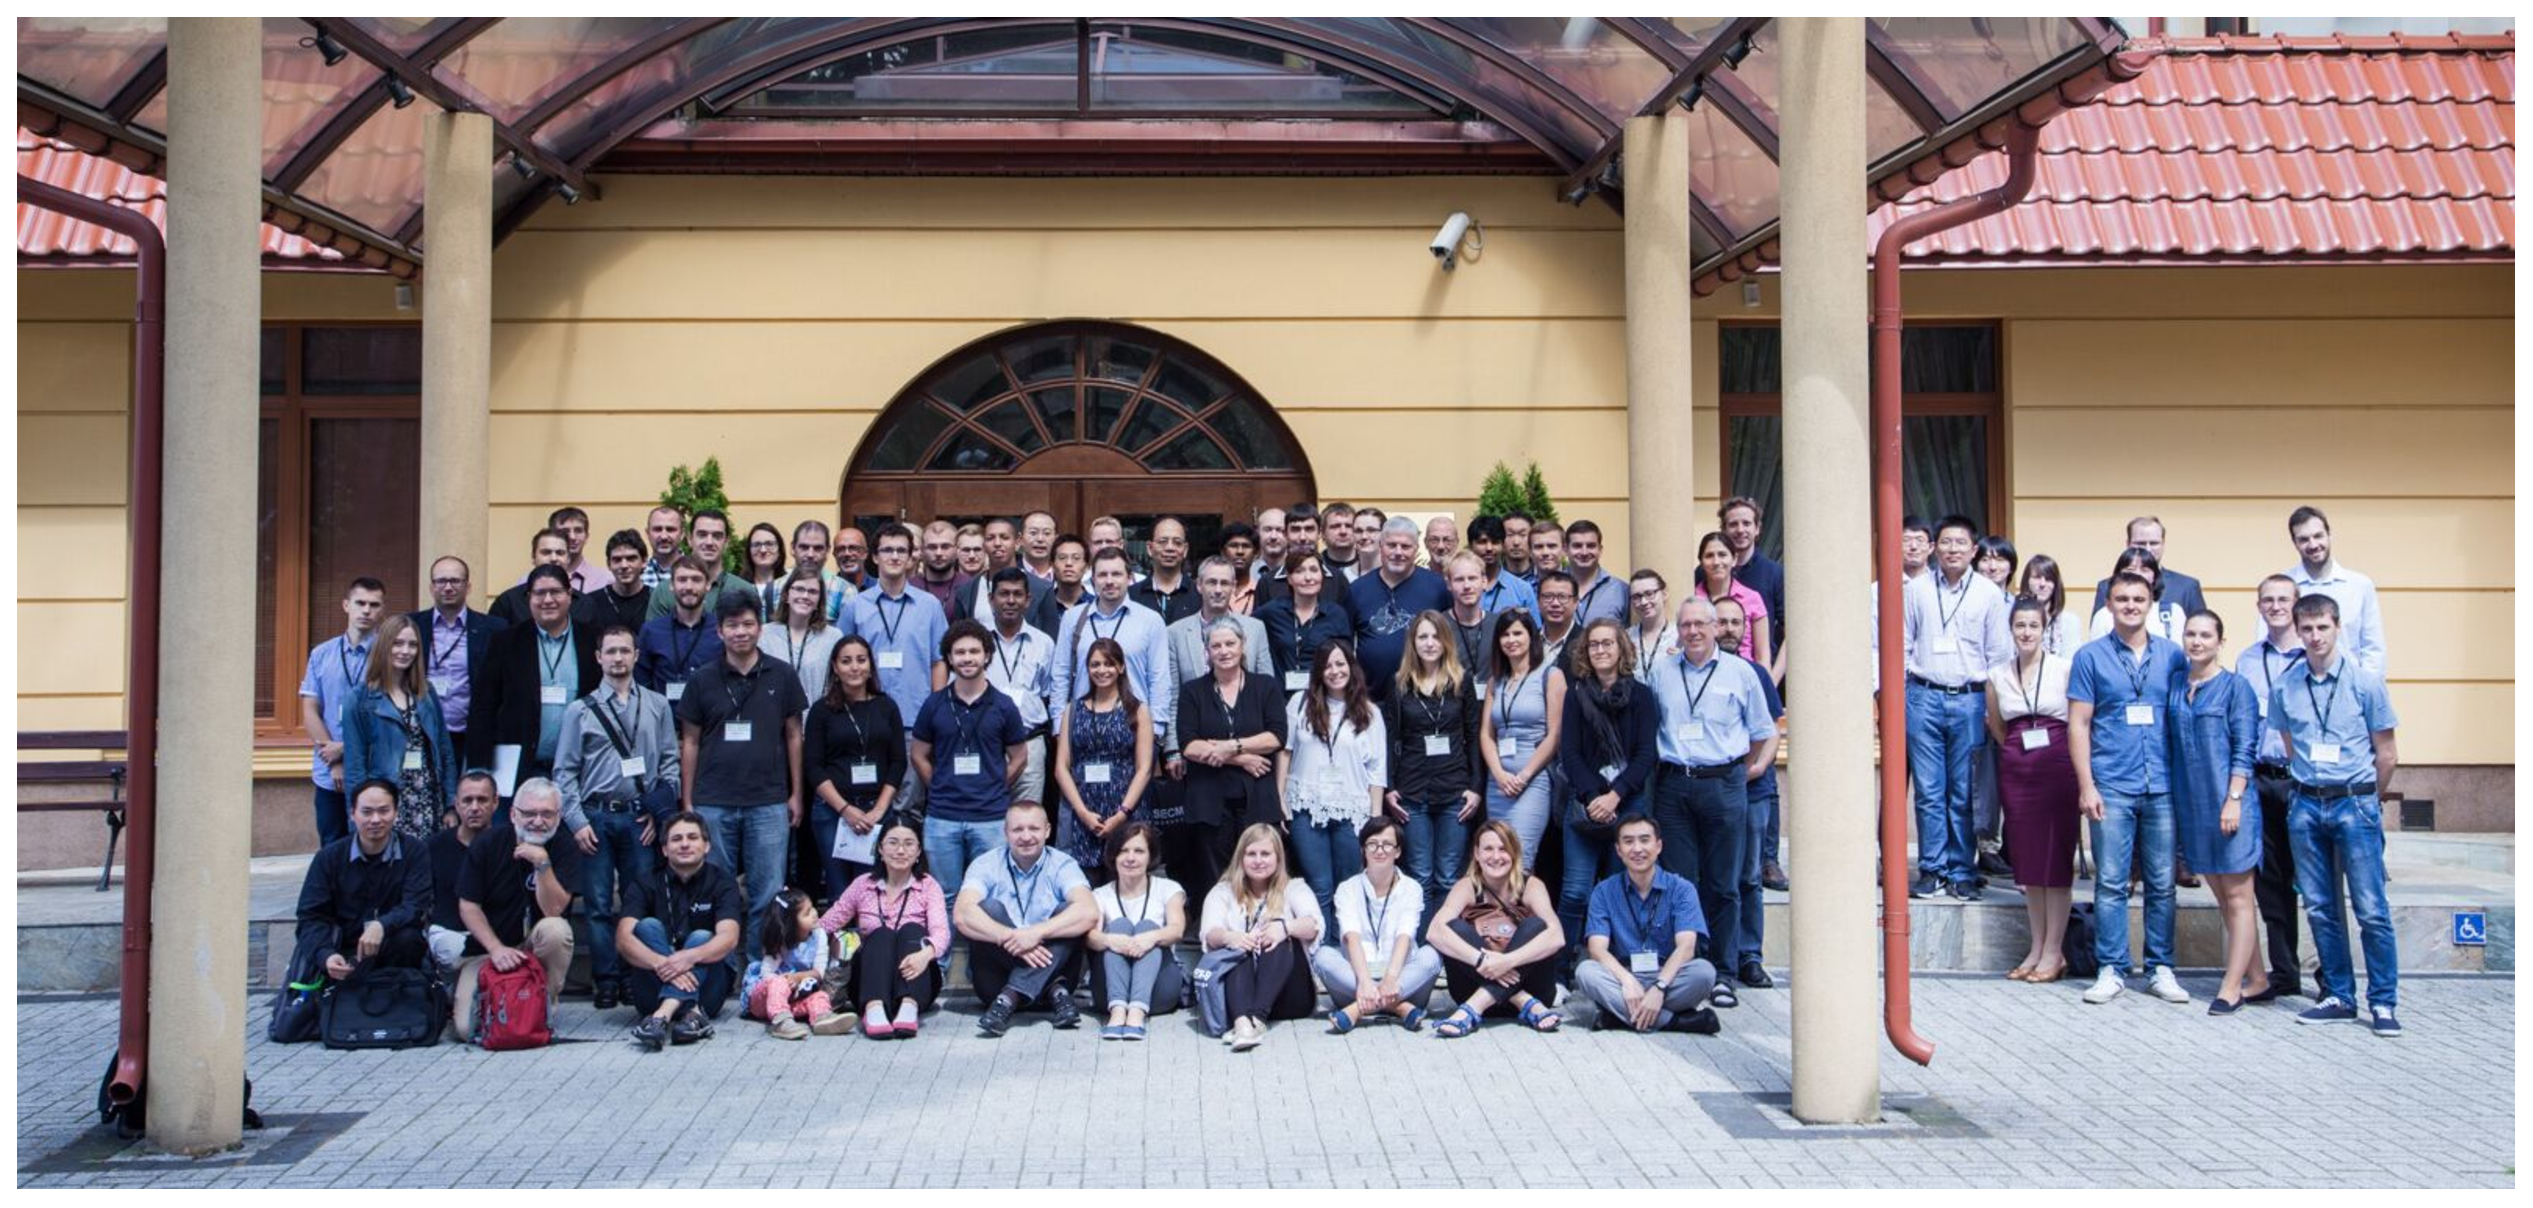
\includegraphics[width=1\textwidth]{poland.eps}
	\frametitle{9th Workshop on Scanning Electrochemical Microscopy and Related Techniques}
	\framesubtitle{Warsaw, Poland, August 13-17, 2017.}
\end{frame}

\begin{frame}[plain]
\centering
Can it be done with amperometric SECM images?
\end{frame}

\begin{frame}[plain]
\centering

\includegraphics[width=0.6\textwidth]{daad.png}
\end{frame}

\begin{frame}
        \centering
        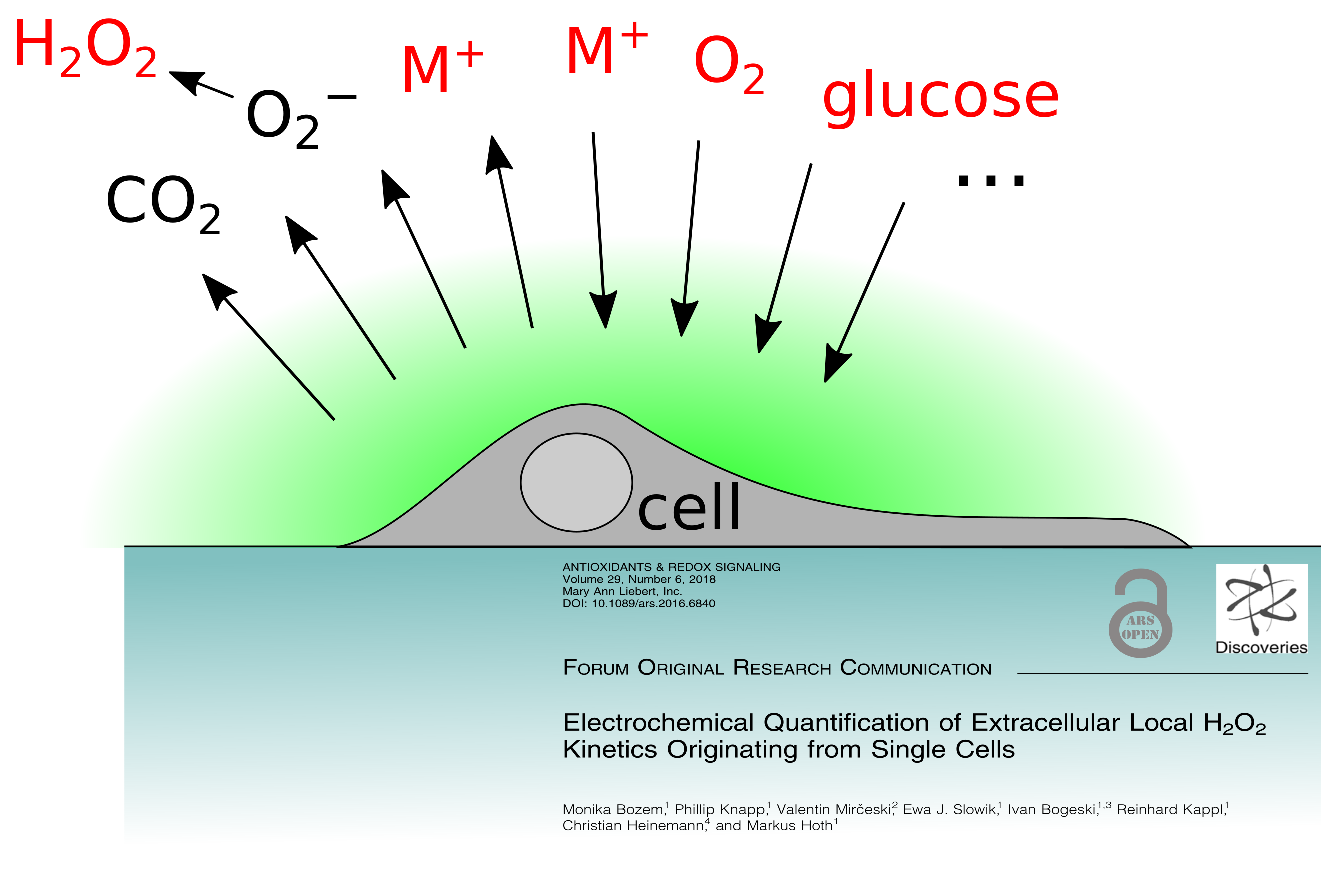
\includegraphics[width=0.9\textwidth]{cell.eps}
        \frametitle{Why would you want to do SECM imaging of a cell?}
	\framesubtitle{It's an easy way to make \emph{in situ}, real-time, selective, non-invasive, high resolution, single cell experiments}
\end{frame}

\begin{frame}
        \centering
        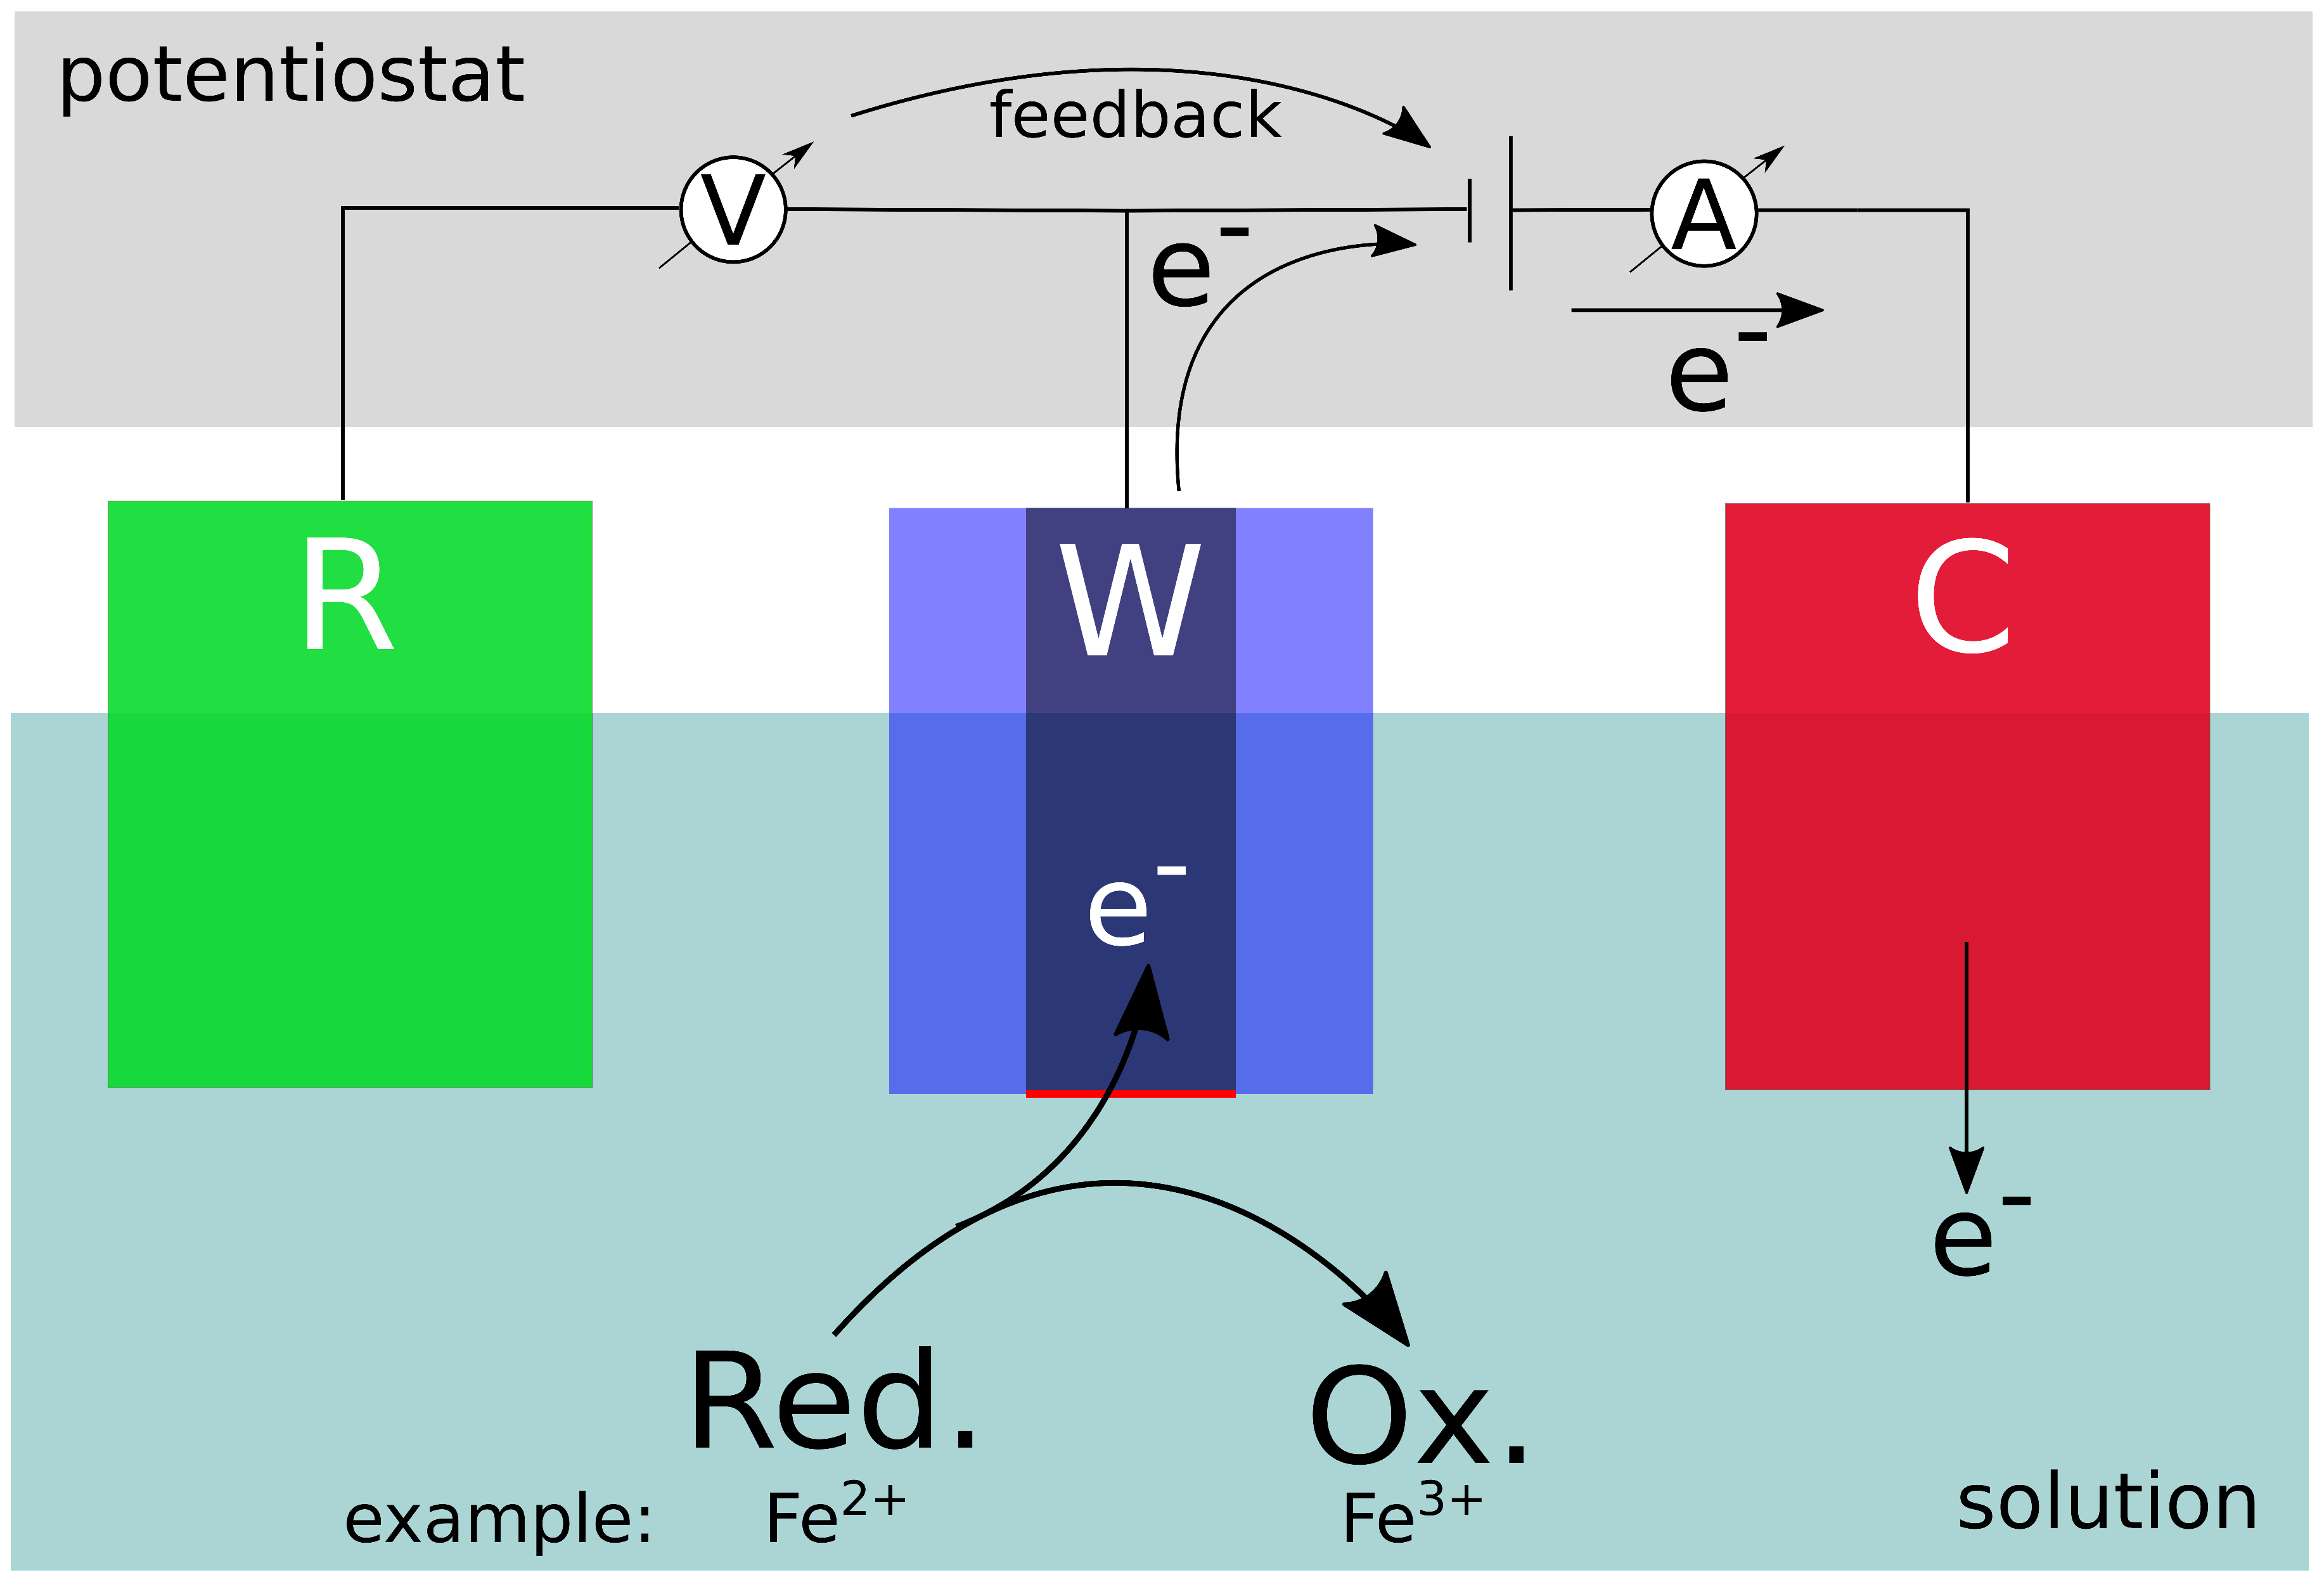
\includegraphics[width=0.9\textwidth]{amperometry.eps}
        \frametitle{The amperometric measuring cell}
\end{frame}

\begin{frame}
        \centering
        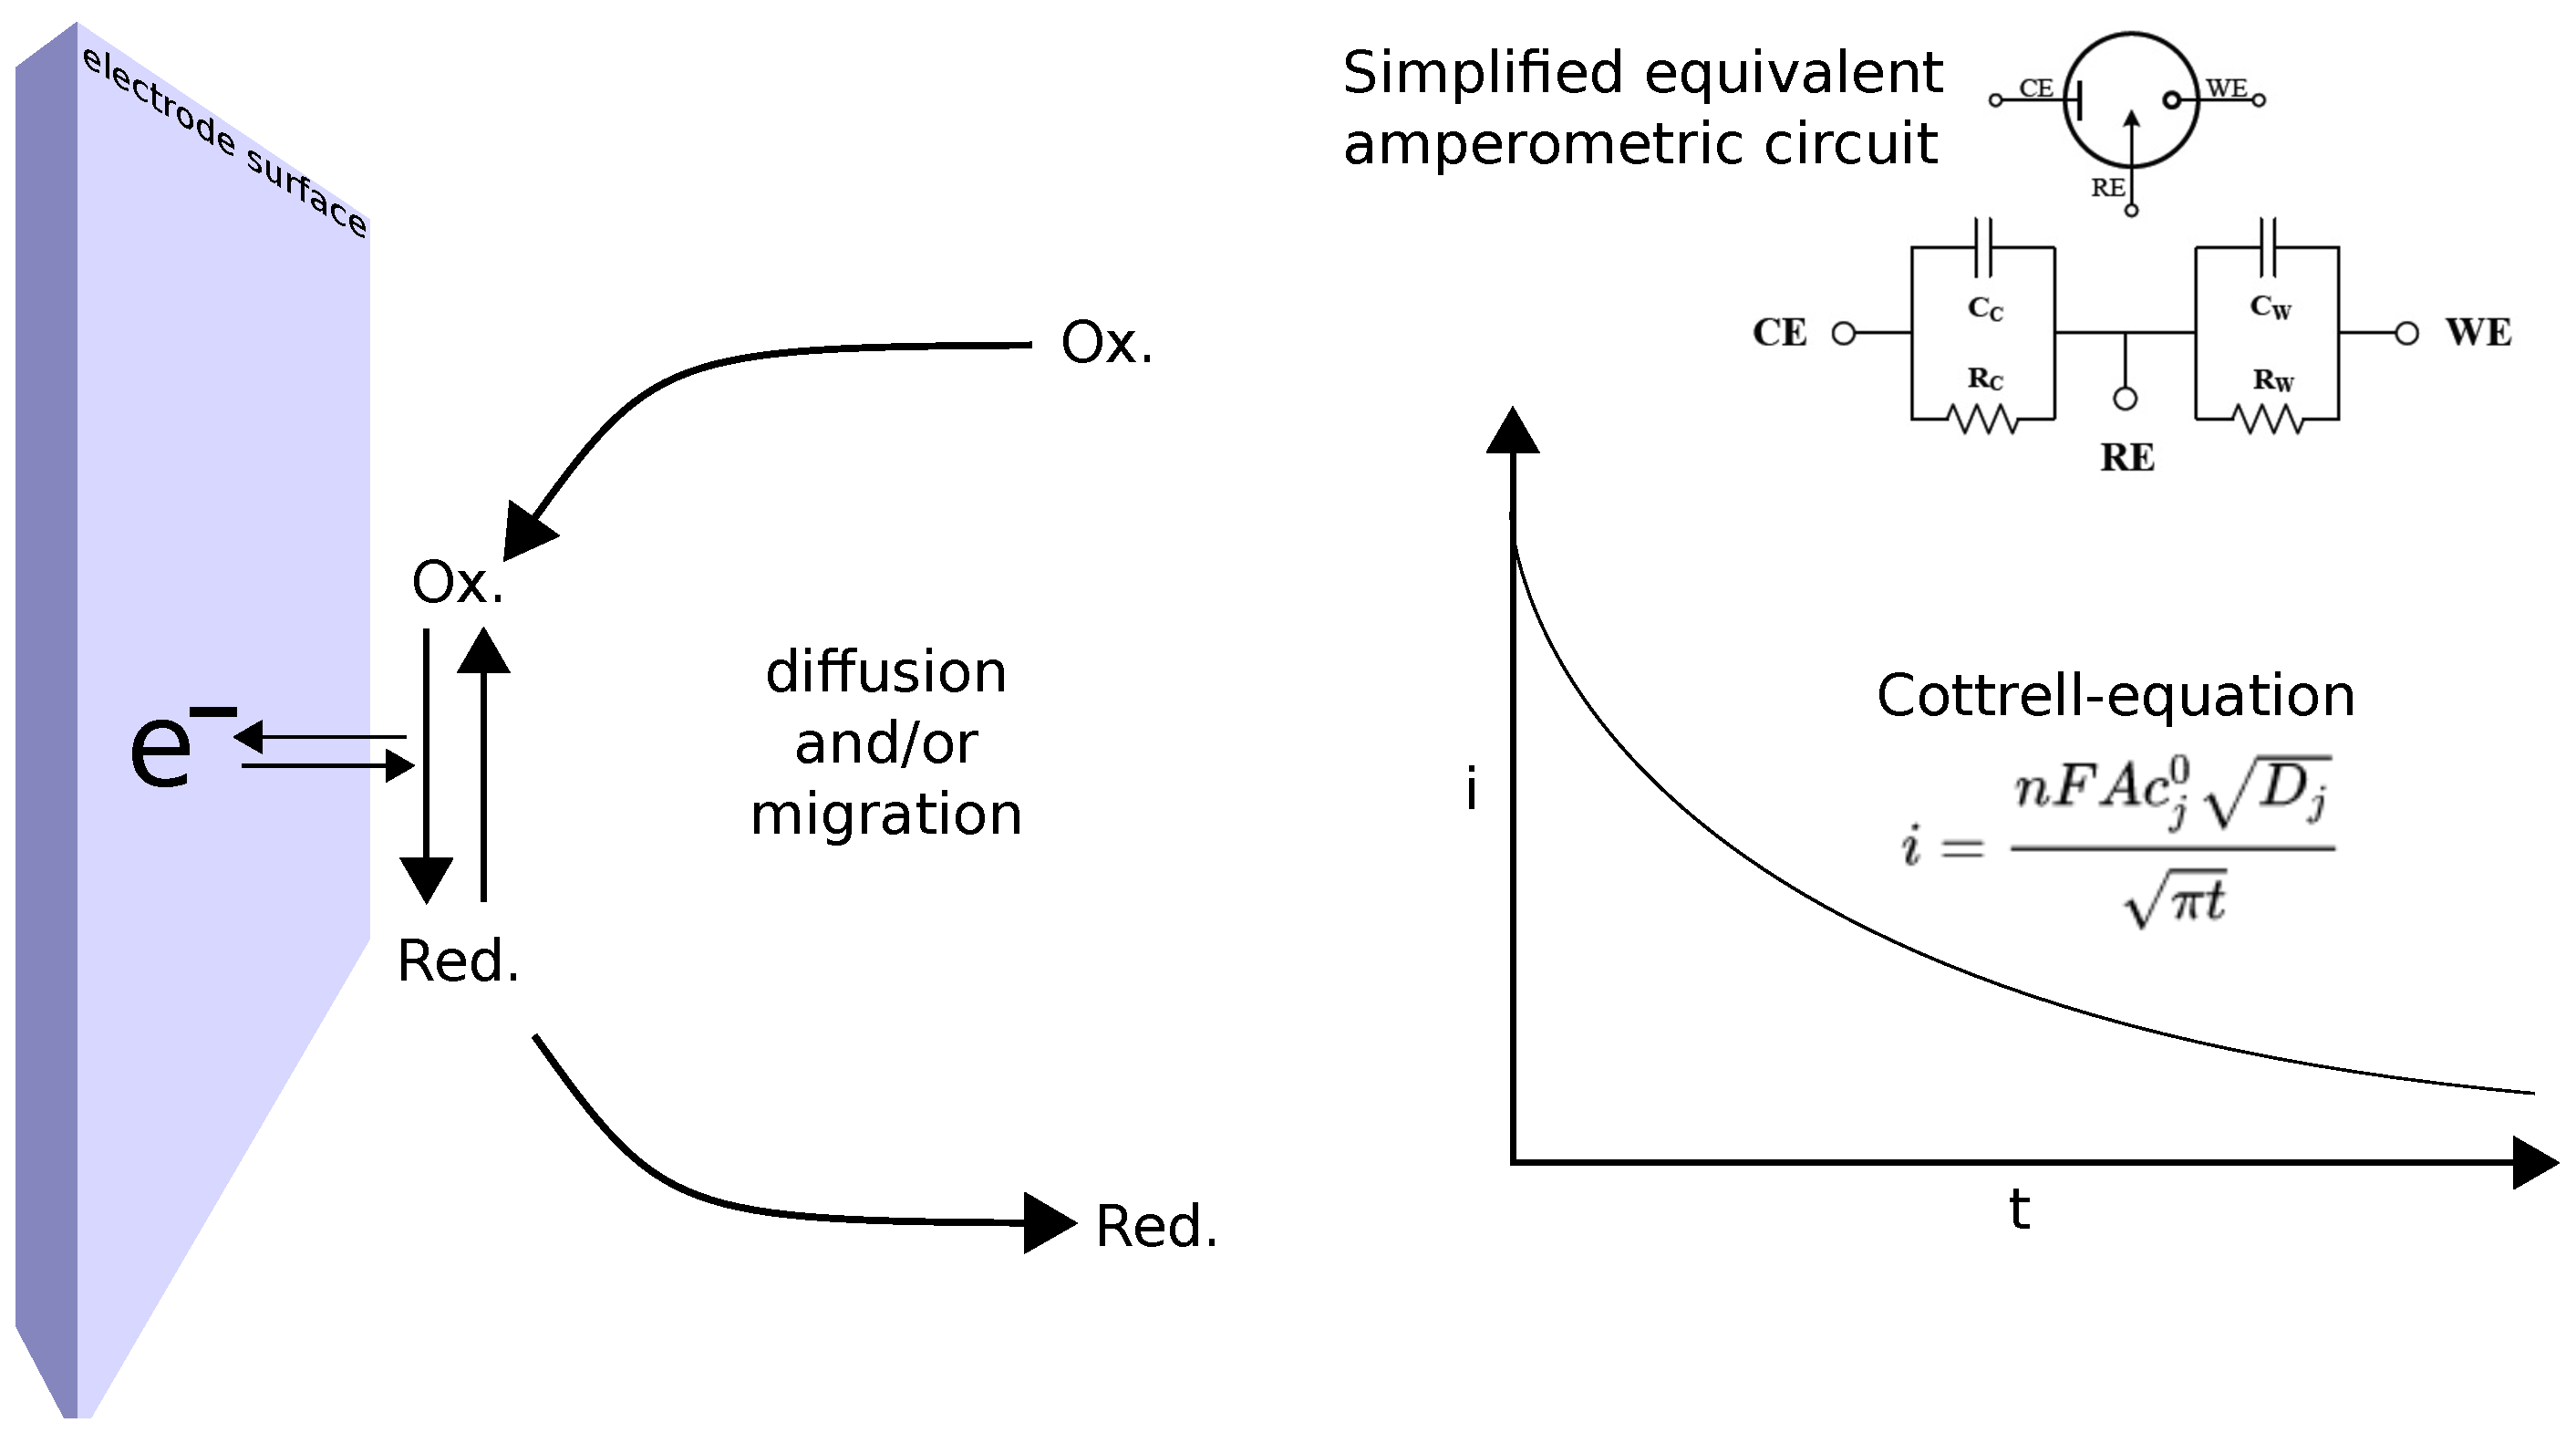
\includegraphics[width=0.9\textwidth]{cottrell.eps}
        \frametitle{Amperometric transient response}
\end{frame}

\begin{frame}
        \centering
        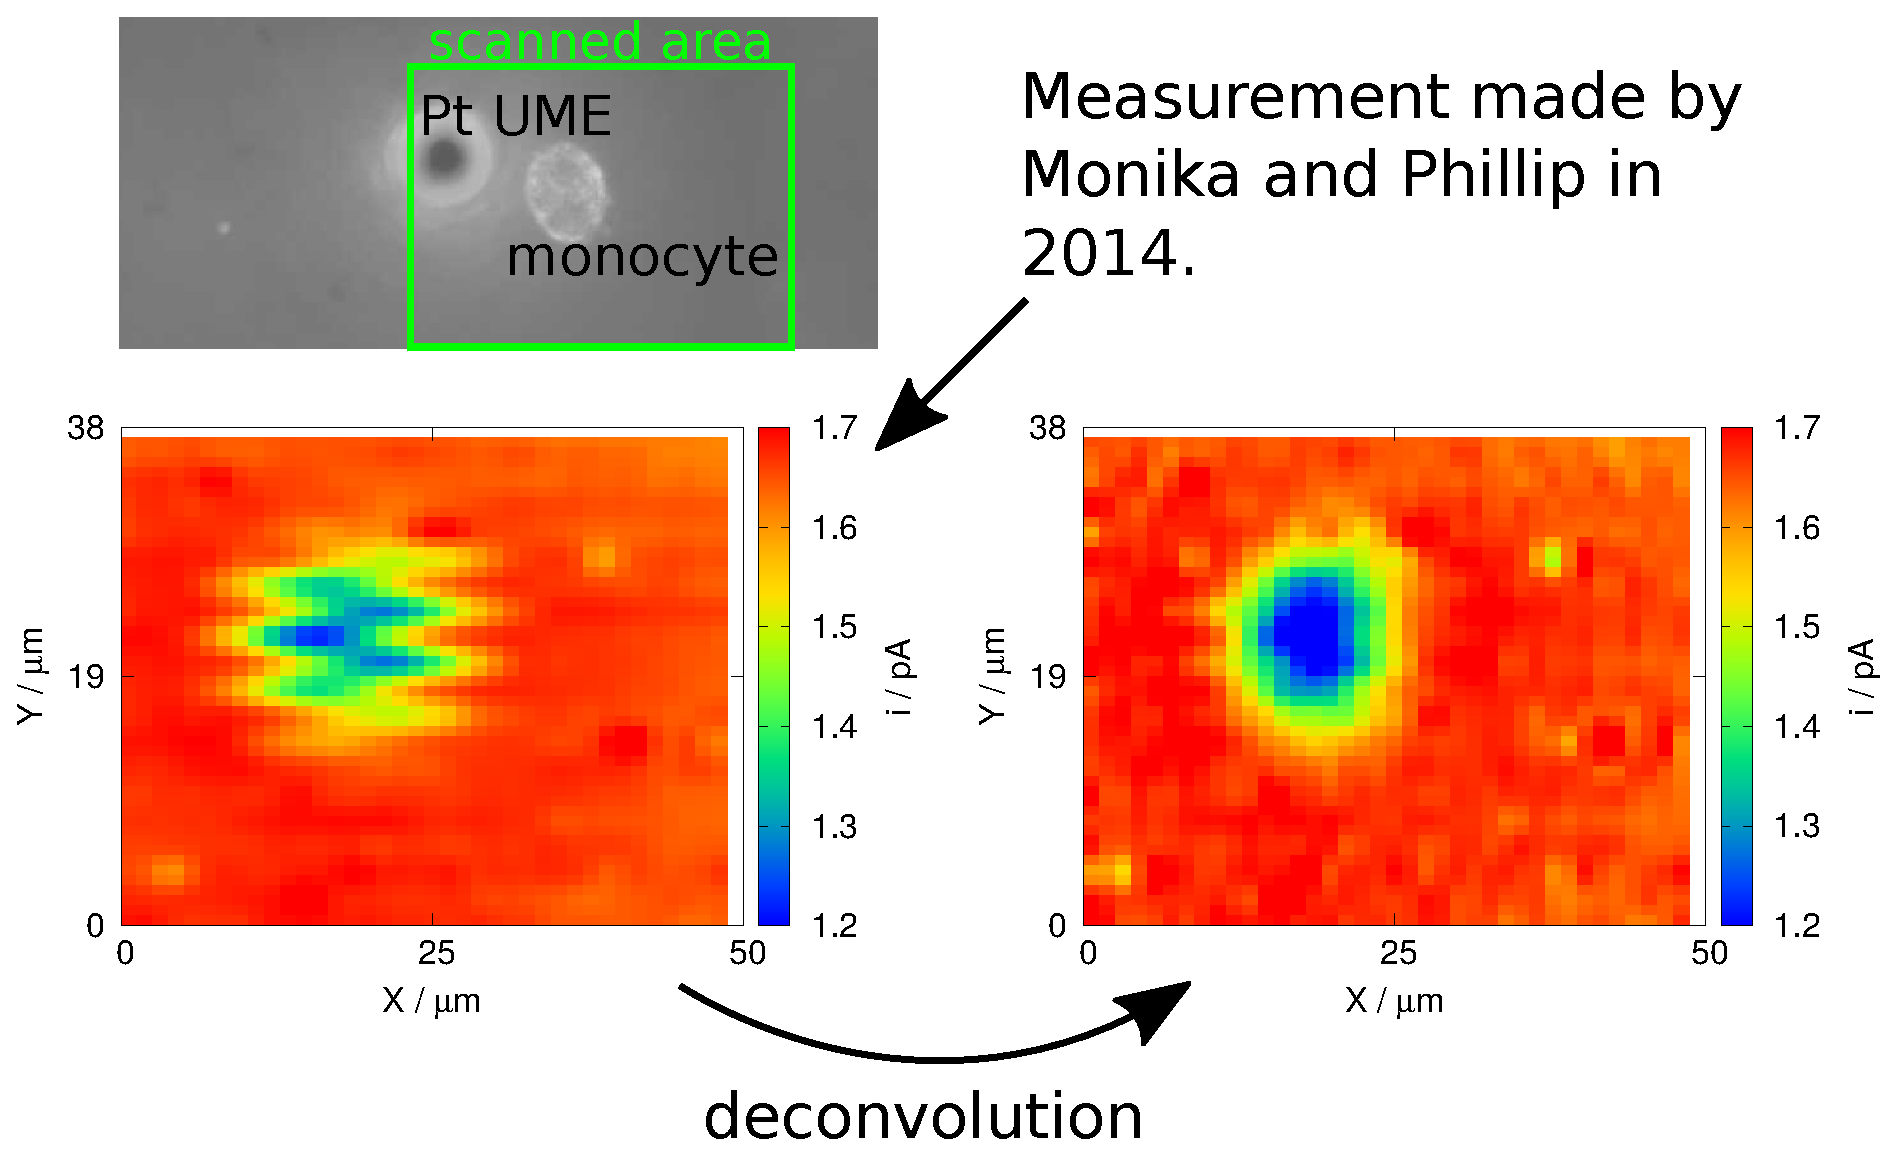
\includegraphics[width=0.9\textwidth]{monocyte.eps}
        \frametitle{Deconvolution of an amperometric image.}
        \framesubtitle{H$_2$O$_2$ oxidation current above a monocyte exposed to extracellular H$_2$O$_2$ (10 $\upmu$M).}
\vfill
%Measurement made by Monika and Phillip in 2014.
\end{frame}

\begin{frame}
        \centering
        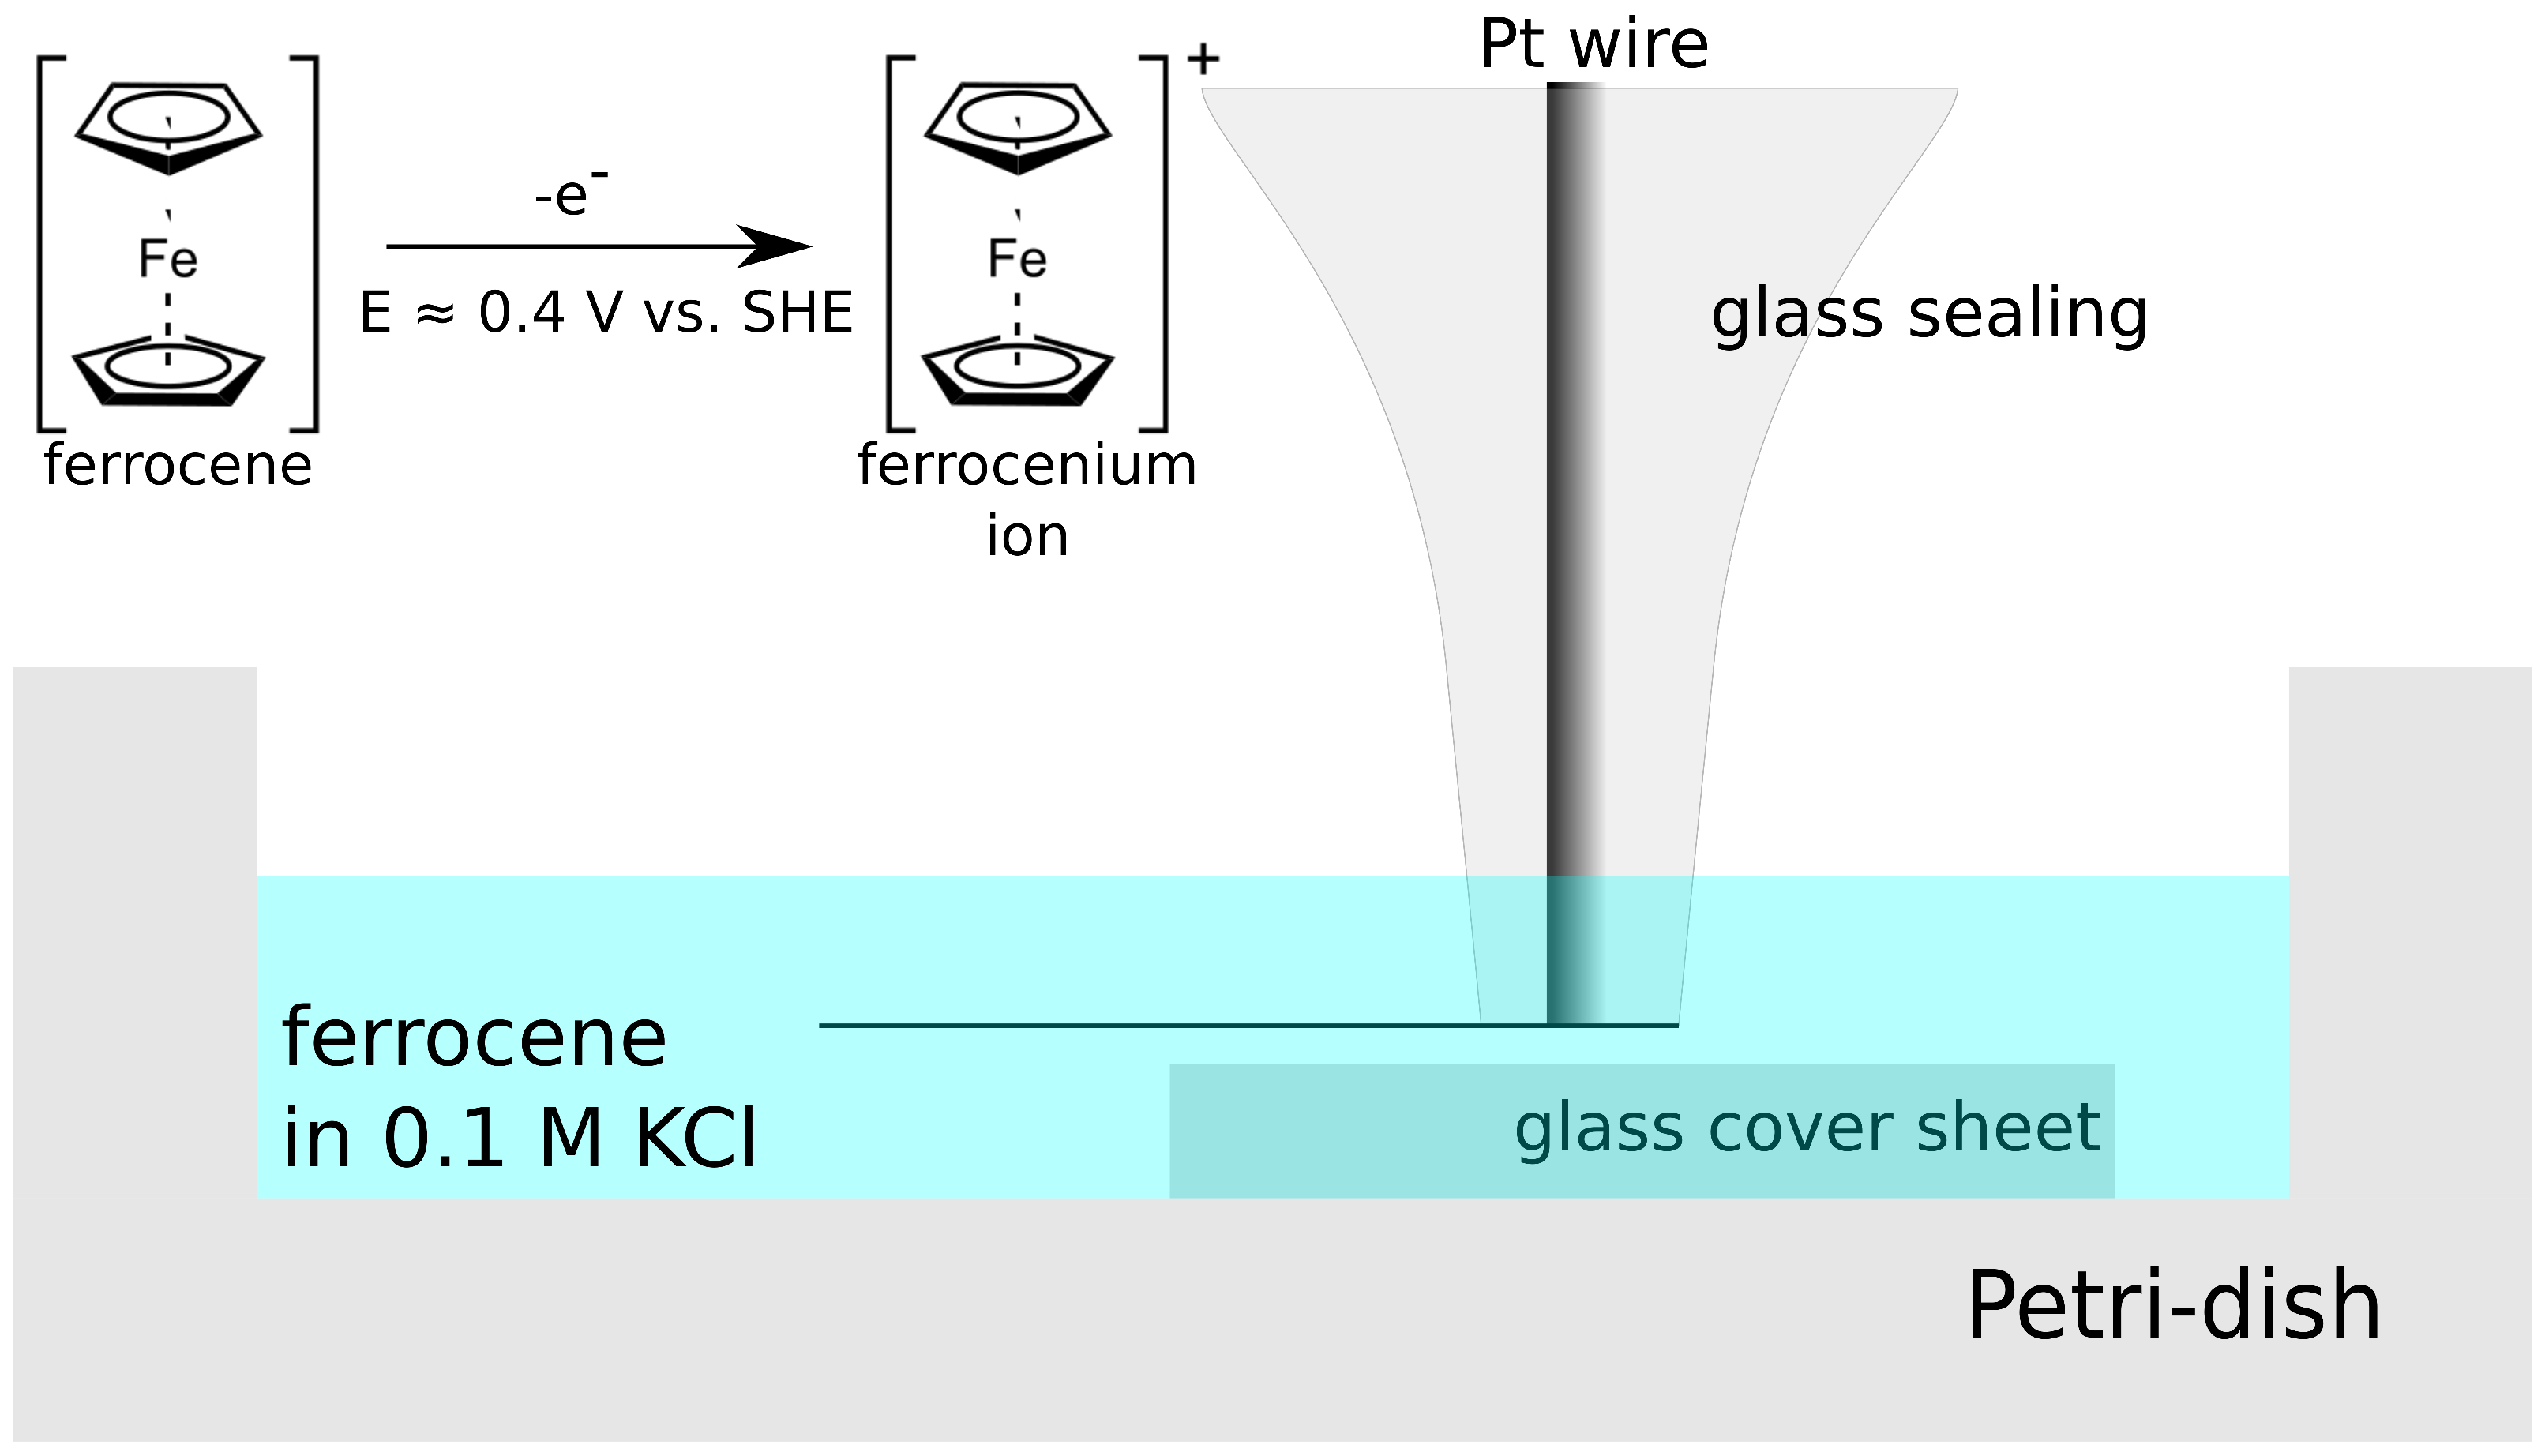
\includegraphics[width=0.9\textwidth]{step.eps}
        \frametitle{Investigating a step response over a glass sheet edge.}
        \framesubtitle{With the ferrocene/ferrocenium system.}
\vfill
\end{frame}

\begin{frame}
        \centering
        \includegraphics[trim = 10mm 60mm 0mm 60mm, clip, width=0.33\textwidth, angle=-90]{1.eps}\includegraphics[trim = 10mm 60mm 0mm 60mm, clip, width=0.33\textwidth, angle=-90]{2_meandered.eps}\includegraphics[trim = 10mm 60mm 0mm 60mm, clip, width=0.33\textwidth, angle=-90]{2_meandered_deconvoluted.eps}

\hspace{1.2cm} 5 $\upmu$m/s \hspace{1.2cm} 10 $\upmu$m/s \hspace{0.2cm} 10 $\upmu$m/s deconvoluted \hfill

\frametitle{Investigating a step response over a glass sheet edge.}
        \framesubtitle{Results.}
\vfill
\end{frame}

\begin{frame}
        \centering
        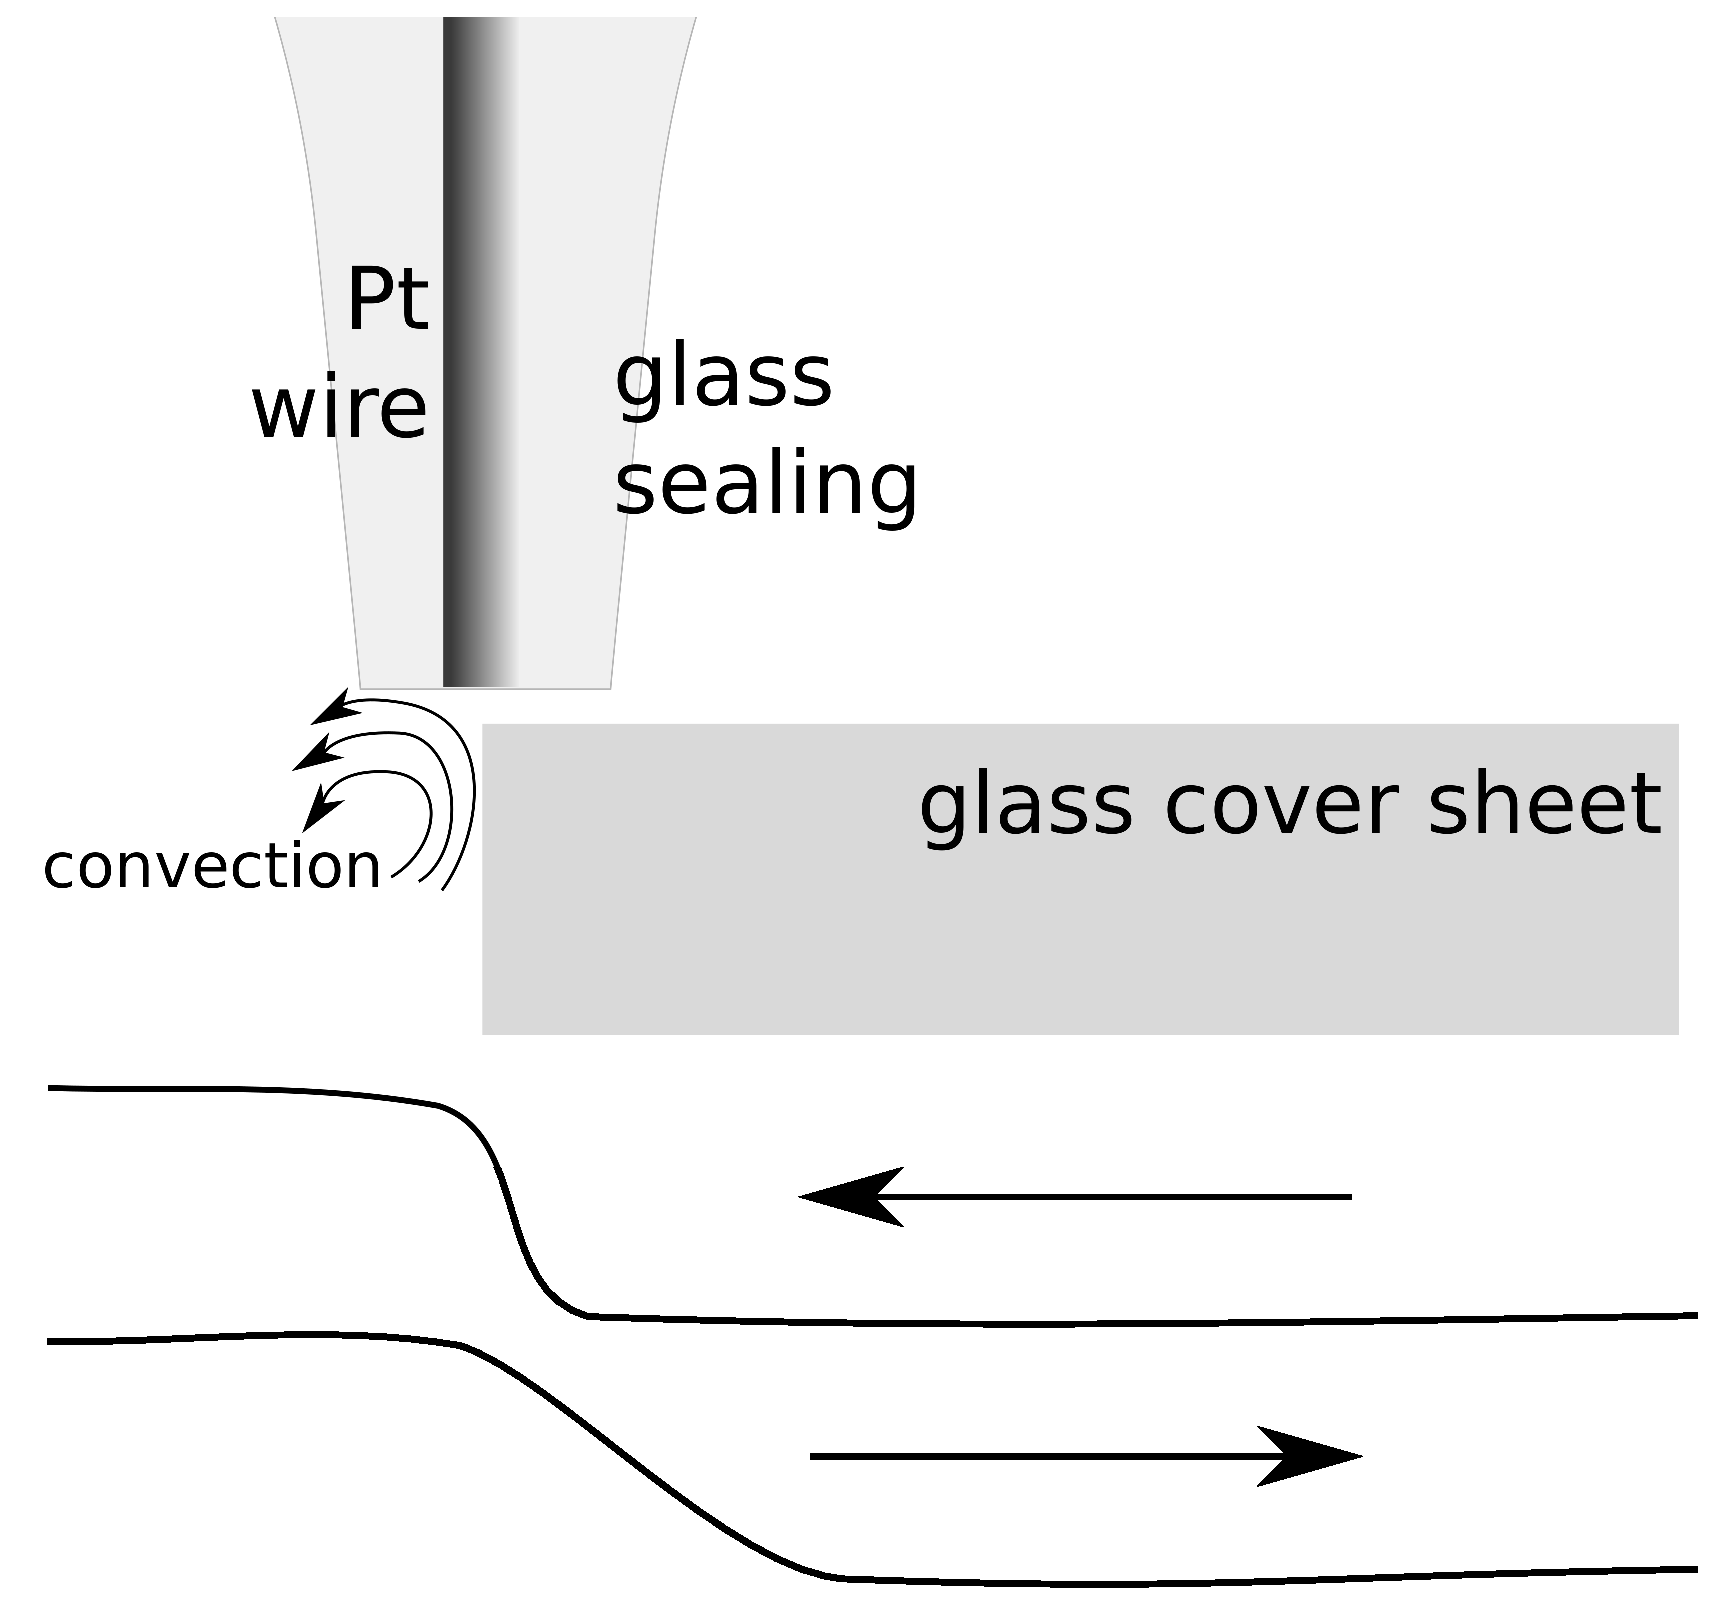
\includegraphics[width=0.6\textwidth]{step_conv.eps}
        \frametitle{Investigating a step response over a glass sheet edge.}
        \framesubtitle{Discrepancy caused by convection.}
\vfill
\end{frame}


\begin{frame}
        \centering
        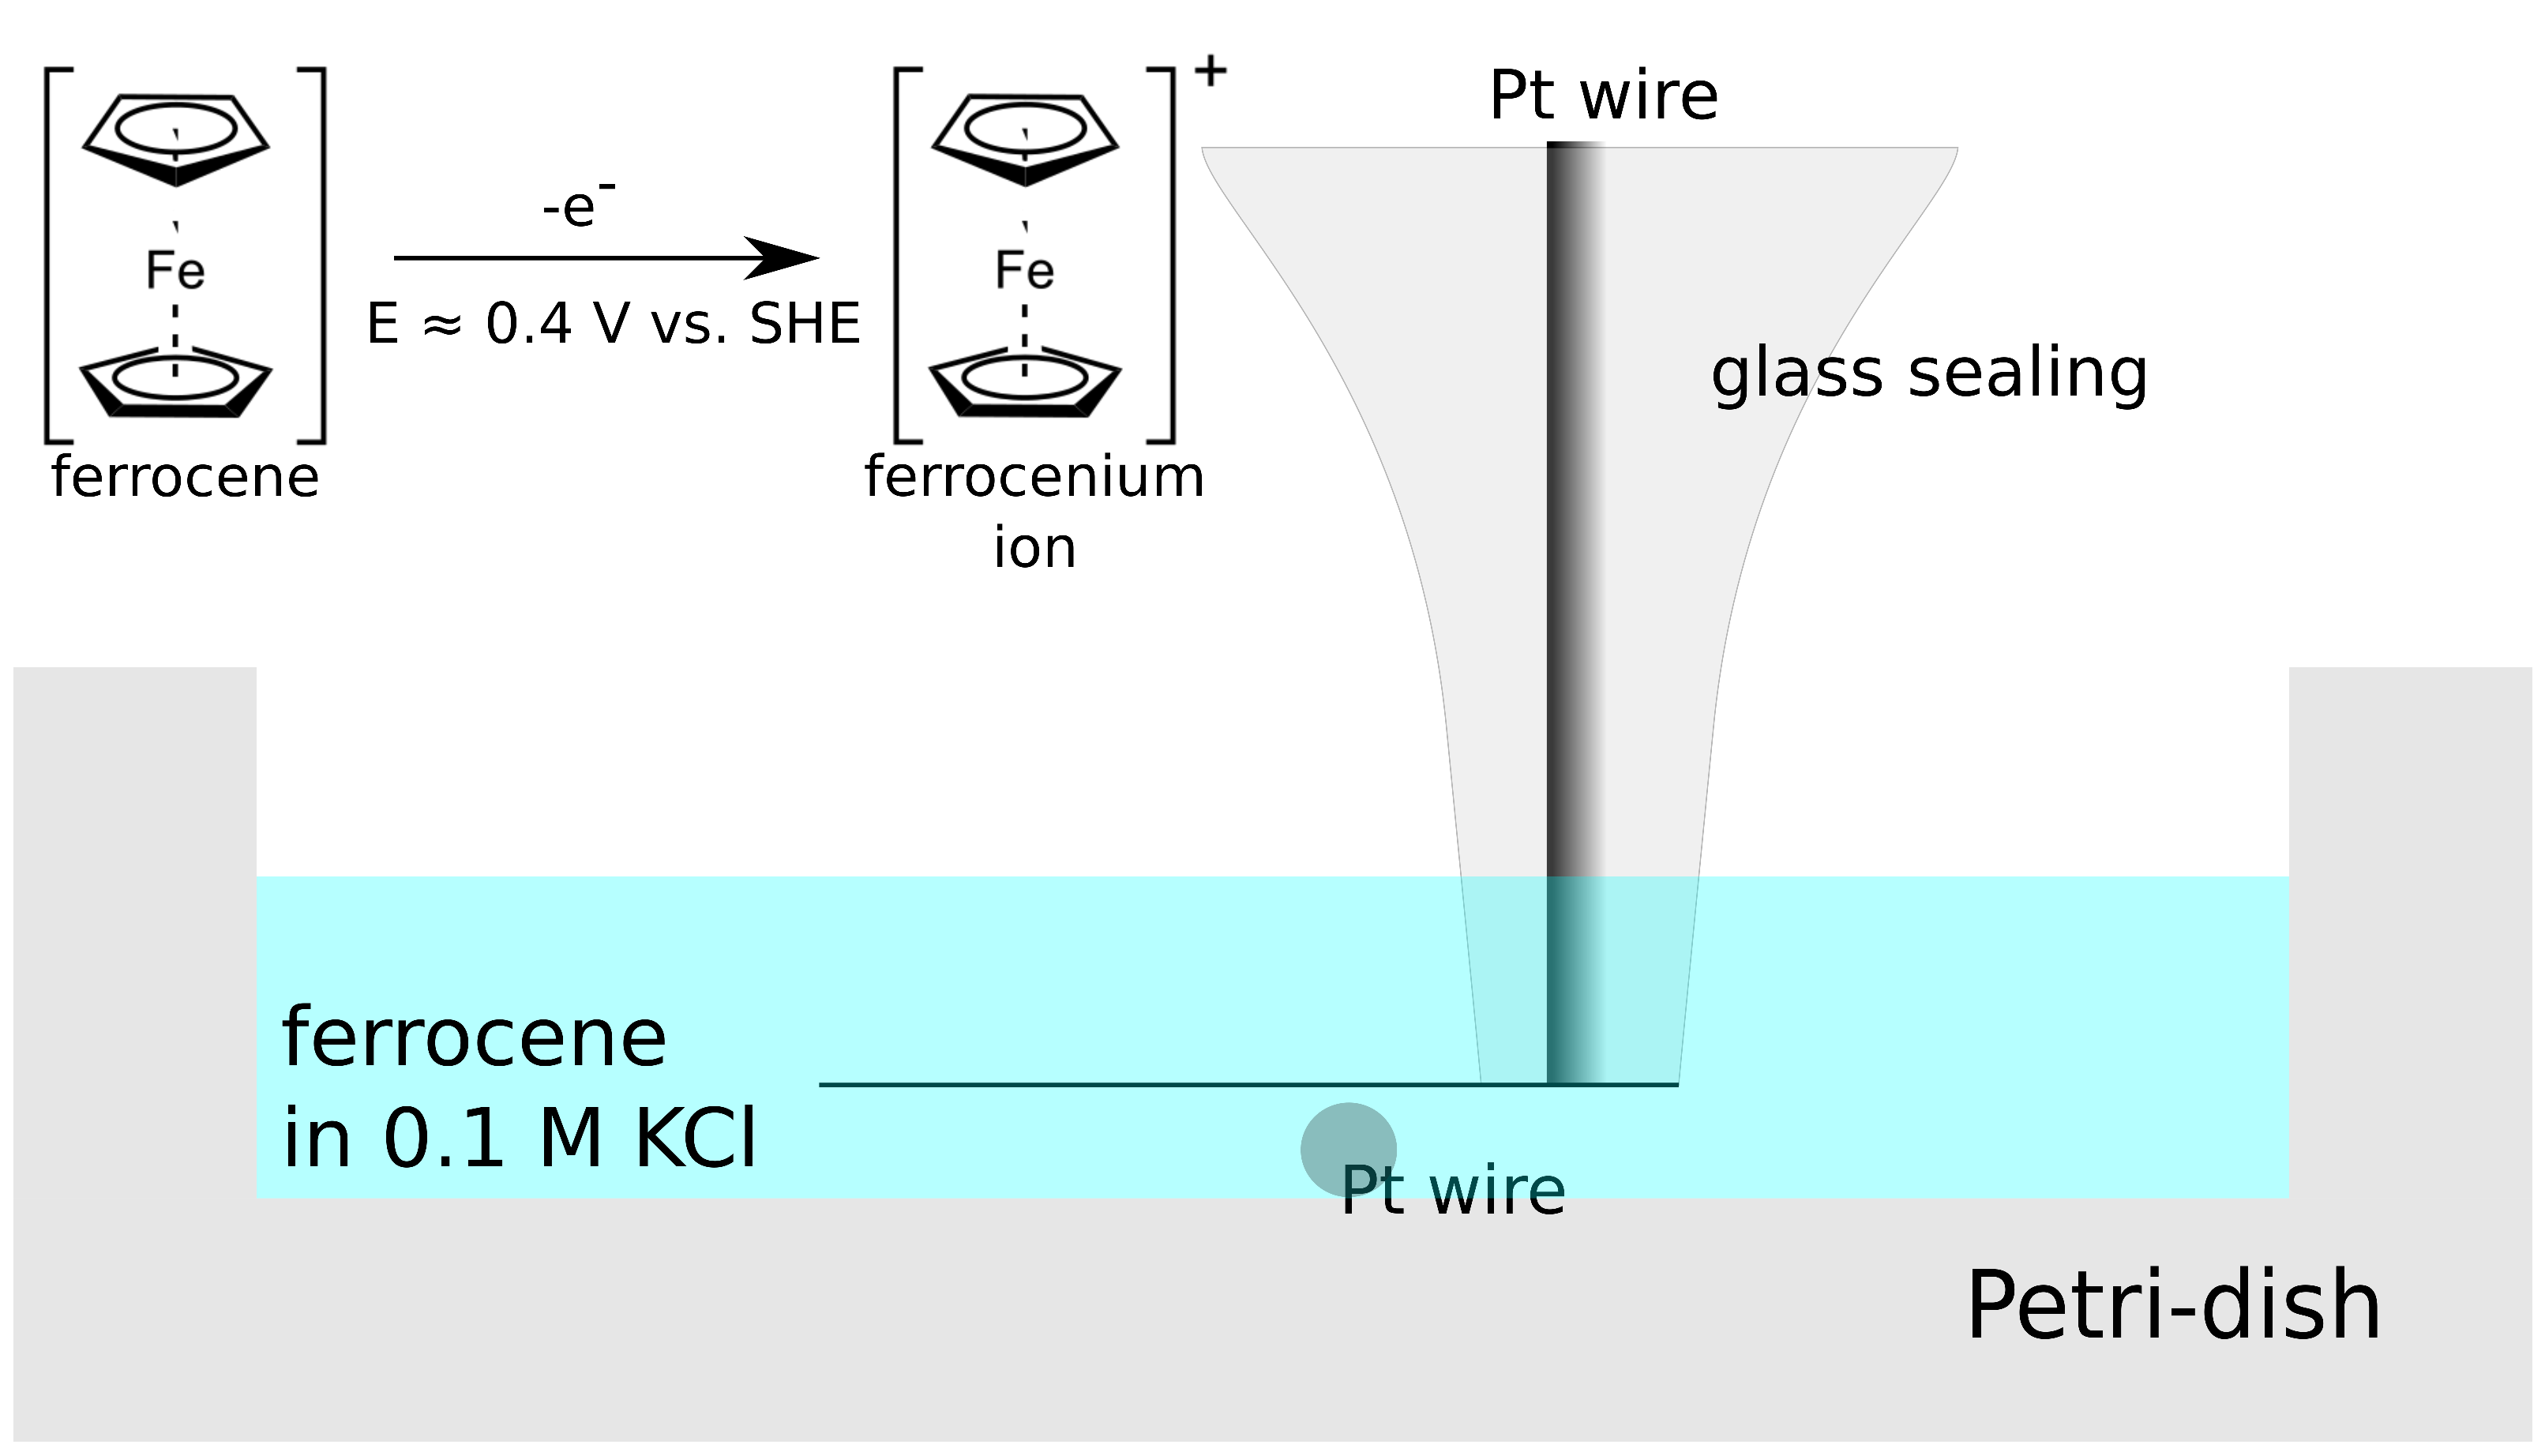
\includegraphics[width=0.9\textwidth]{wire.eps}
        \frametitle{Investigating a step response over a d = 10 $\upmu$m Pt wire.}
        \framesubtitle{With the ferrocene/ferrocenium system.}
\vfill
\end{frame}

\begin{frame}
        \centering
        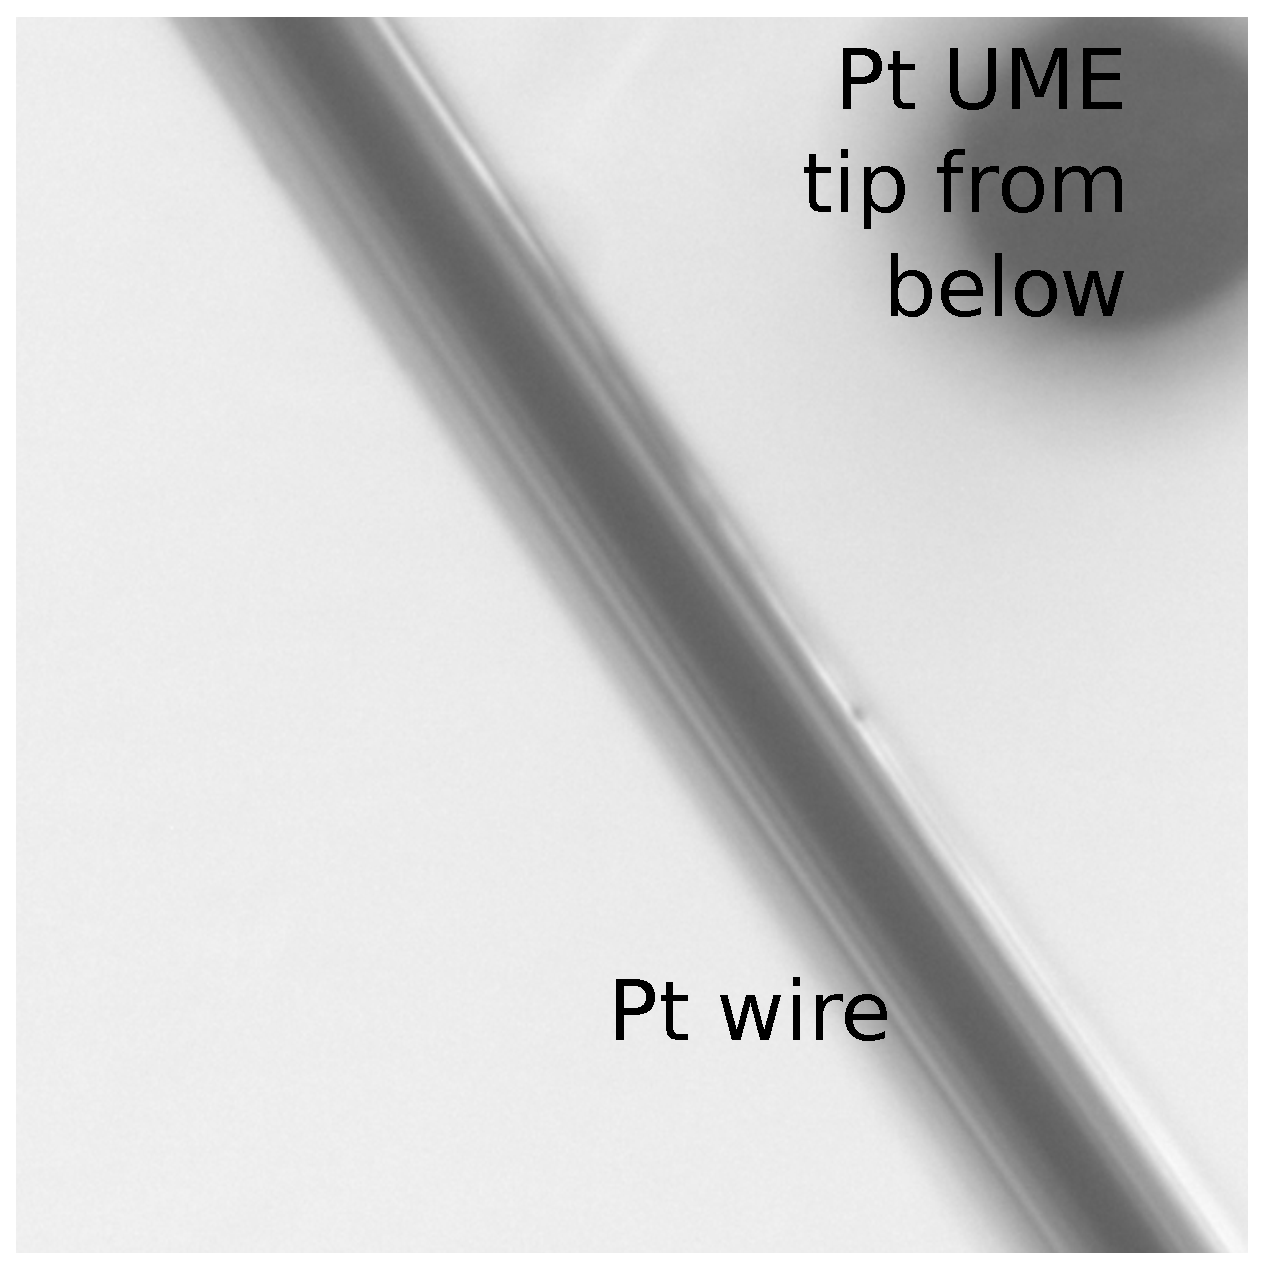
\includegraphics[width=0.6\textwidth]{wire_photo.eps}
        \frametitle{Investigating a step response over a d = 10 $\upmu$m Pt wire.}
        \framesubtitle{Microphoto of the model system from below.}
\vfill
\end{frame}


\begin{frame}
        \centering
        \includegraphics[trim = 10mm 10mm 0mm 10mm, clip, width=0.4\textwidth, angle=-90]{7.eps}\includegraphics[trim = 10mm 30mm 0mm 10mm, clip, width=0.4\textwidth, angle=-90]{7_deconvoluted.eps}

\hspace{1.4cm} 10 $\upmu$m/s \hspace{3cm} 10 $\upmu$m/s deconvoluted

\frametitle{Investigating a step response over a d = 10 $\upmu$m Pt wire.}
        \framesubtitle{Results.}
\vfill
\end{frame}


\begin{frame}
        \centering
        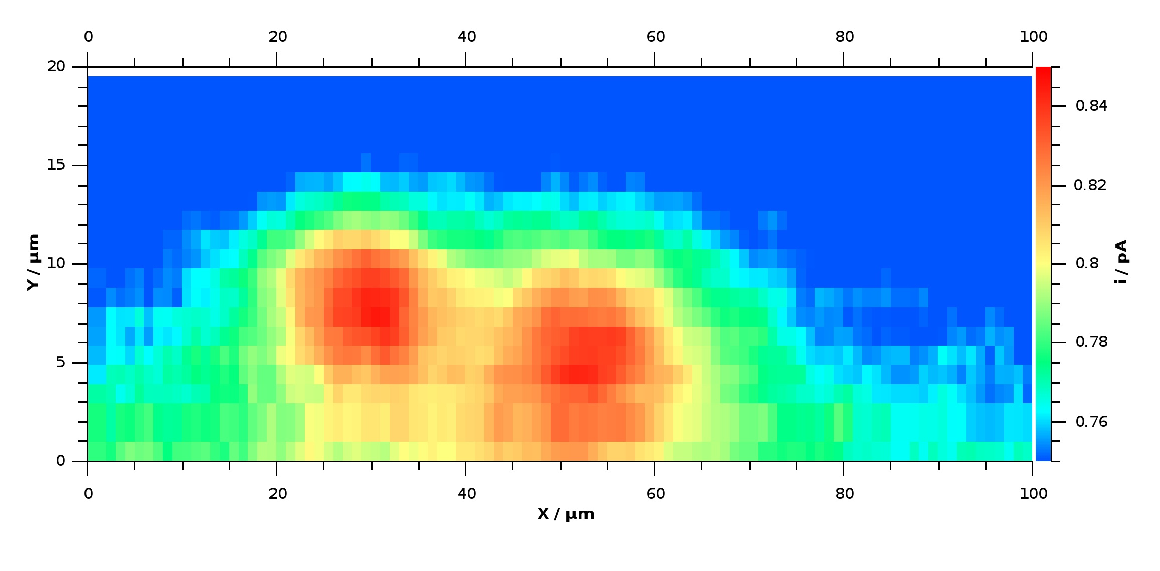
\includegraphics[width=0.5\textwidth]{original.eps}
	
	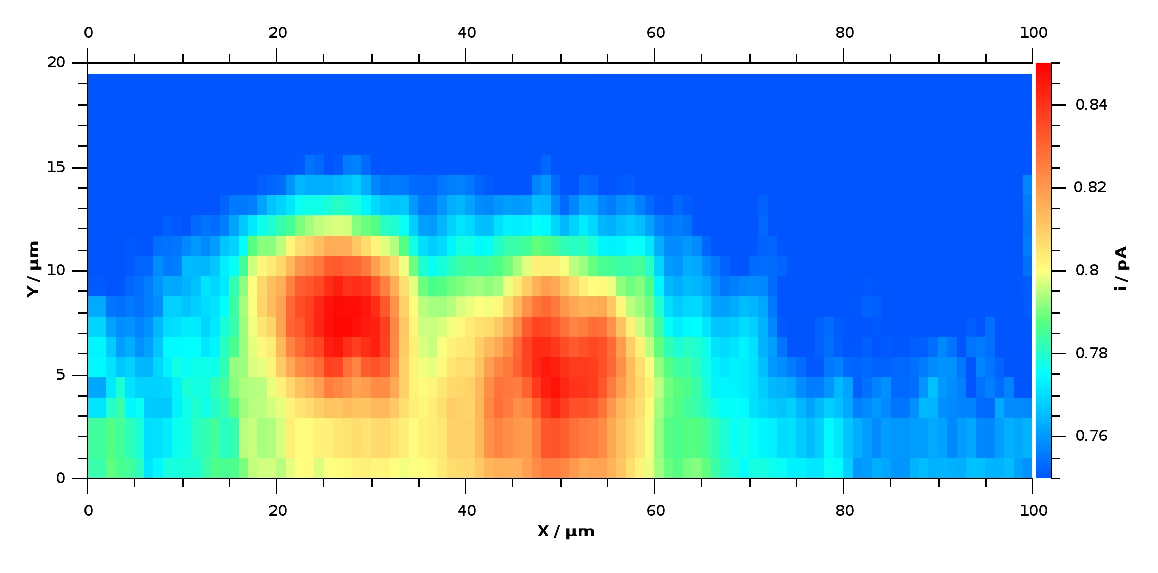
\includegraphics[width=0.5\textwidth]{deconvoluted.eps}

%\hspace{1.2cm} 5 $\upmu$m/s \hspace{1.2cm} 10 $\upmu$m/s \hspace{0.2cm} 10 $\upmu$m/s deconvoluted \hfill

\frametitle{H$_2$O$_2$ measurement over a TPA stimulated monocyte.}
        \framesubtitle{Results.}

\vfill
Top image: original measurement, made by Monika in 2014. Scanning speed was 2 $\upmu$m/s. Bottom image: deconvoluted image.
\end{frame}


\begin{frame}
        \centering
        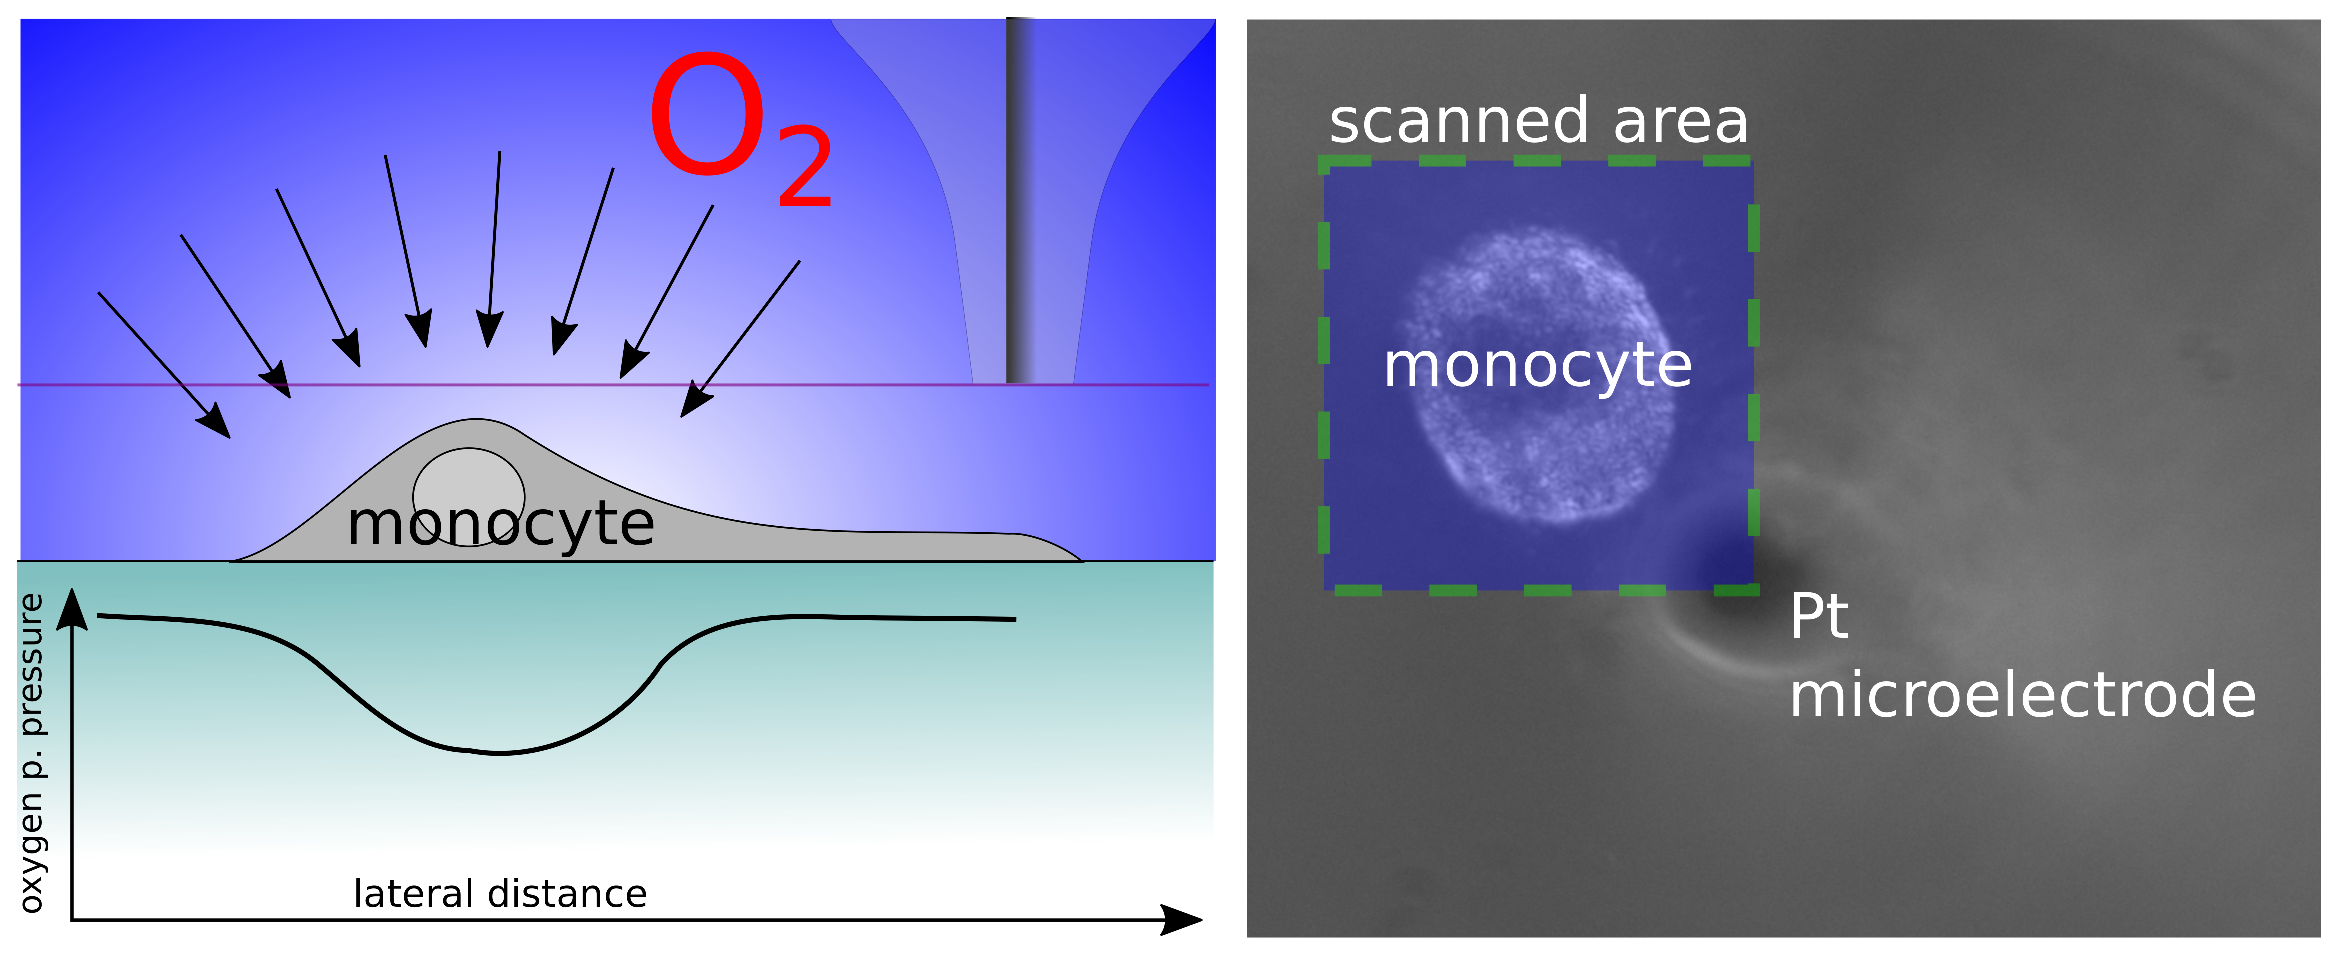
\includegraphics[width=1\textwidth]{oxygen.eps}

\frametitle{Oxygen reduction current above a monocyte.}
\framesubtitle{Experimental setup.}
\end{frame}




\begin{frame}
        \centering
        \includegraphics[trim = 10mm 20mm 0mm 20mm, clip, width=0.4\textwidth, angle=-90]{9_41.eps}\includegraphics[trim = 10mm 20mm 0mm 20mm, clip, width=0.4\textwidth, angle=-90]{9_41_meandered_deconvoluted.eps}

%\hspace{1.2cm} 5 $\upmu$m/s \hspace{1.2cm} 10 $\upmu$m/s \hspace{0.2cm} 10 $\upmu$m/s deconvoluted \hfill

\frametitle{Oxygen reduction current above a monocyte.}
        \framesubtitle{Results.}
\vfill
\end{frame}




\begin{frame}
\frametitle{Conclusion}
%\scriptsize
\begin{enumerate}
\item \textbf{SECM is a powerful tool. Many systems can be studied best with this technique.}
\item \textbf{However, it suffers from low scan speeds and high distortion.}
\item \textbf{Previously I have worked out a deconvolution technique to solve this problem for potentiometric SECM.}
\item \textbf{During my stay here I have worked out a similar method for amperometric SECM.}
\item \textbf{I have used the technique to restore images recorded by Monika and Phillip previously.}
\item \textbf{I have introduced single cell oxygen measurements here with the SECM, and successfully applied the deconvolution to those images as well.}

\end{enumerate}
\end{frame}

\begin{frame} %[plain]

\centering
\frametitle{Thank you!}

Dr. Monika Bozem

Prof. Dr. Markus Hoth

Phillip Knapp

Katerina Stankoska

Rüdiger Stumpf

Staff of CIPMM

\vspace{1 cm}

DAAD

\vspace{1 cm}

Thank you for your kind attention!

	%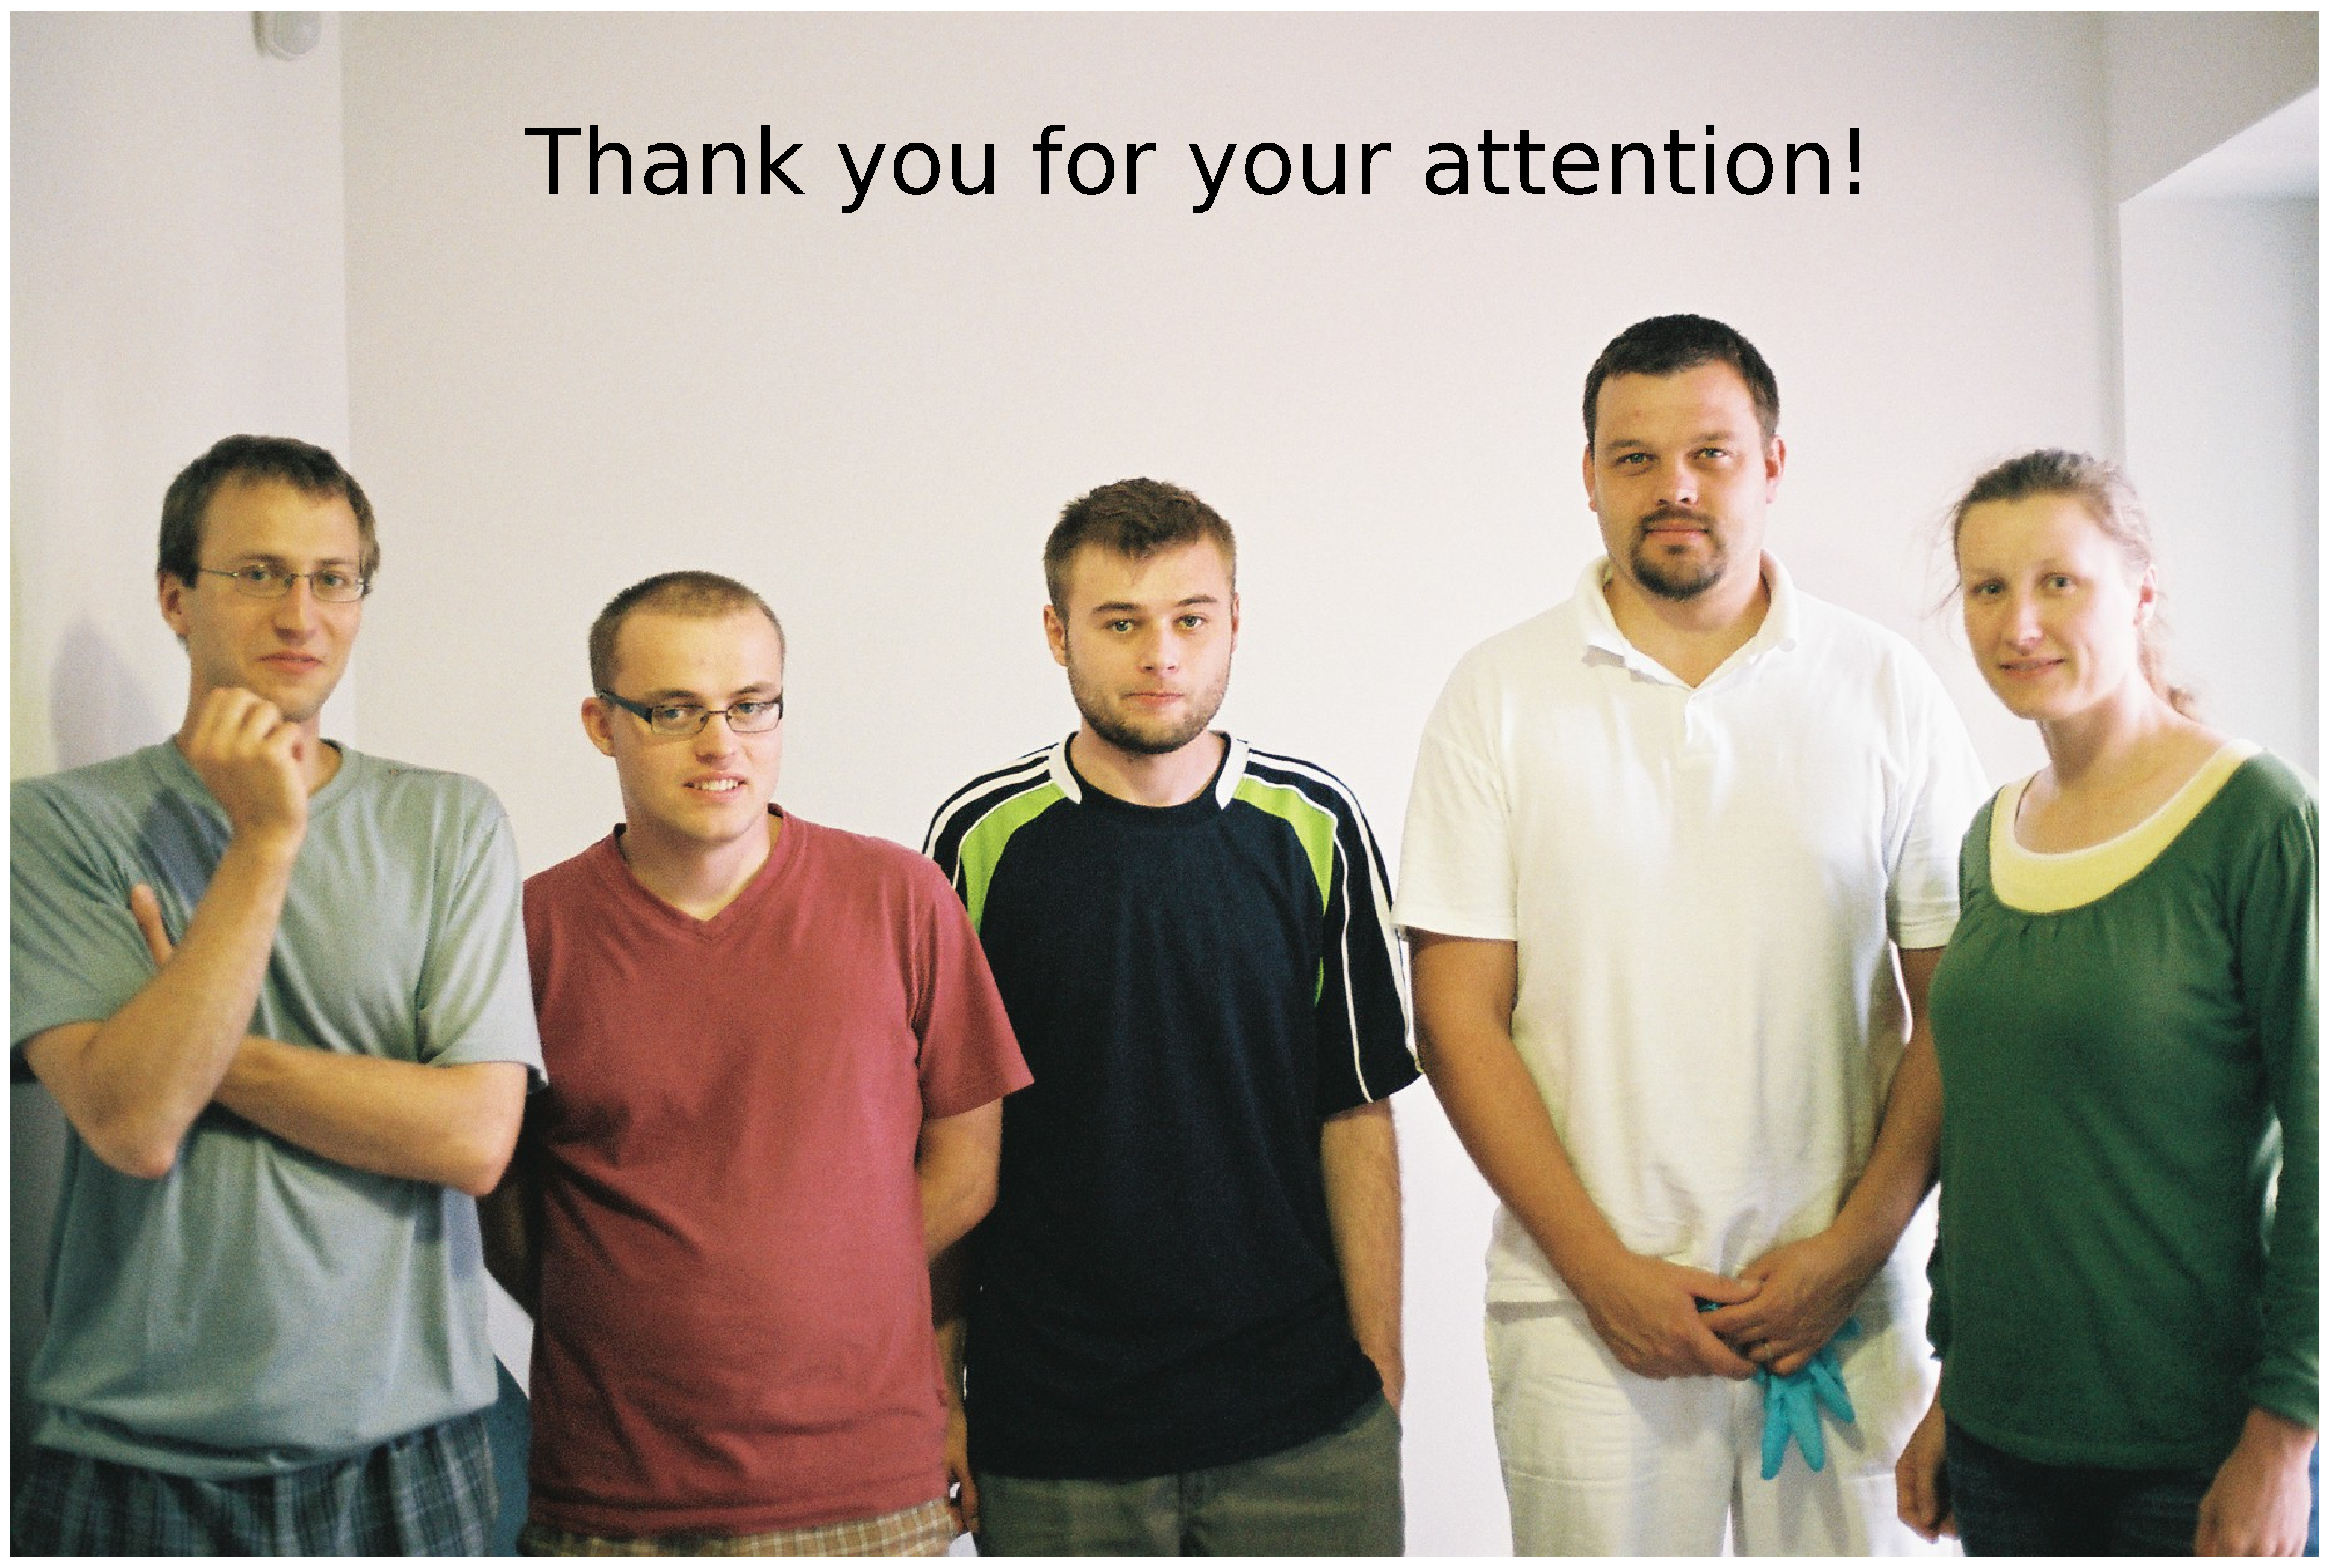
\includegraphics[width=1\textwidth]{thankyou.eps}
\end{frame}

\end{document}
